\begin{document}

\subsection{フロント管理画面}

\subsubsection{フロントTOP画面}
 図\ref{fig:frontTop}にフロントTOP画面を示す.

\begin{figure}[H]
 \centering
   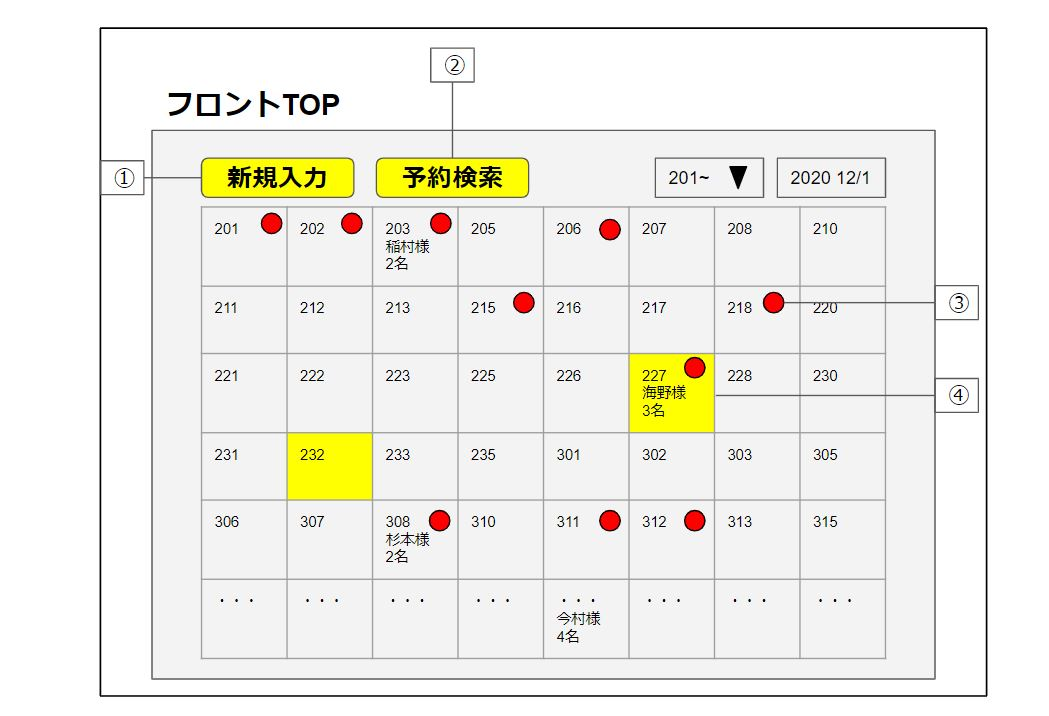
\includegraphics[width=120mm]{UI_front/frontTop.jpg}
 \caption{フロントTOP画面}
 \label{fig:frontTop}
\end{figure}

\begin{enumerate}
\renewcommand{\labelenumi}{\textcircled{\scriptsize \theenumi}}
\item 新規予約入力\\ 新規予約を押すこで,図\ref{fig:frontR1},図\ref{fig:frontR2}に示す予約入力画面に遷移する.
\item 予約検索\\ 予約検索を押すことで,図\ref{fig:frontS}に示す予約検索画面に遷移する.
\item 清掃情報\\未清掃の場合,赤の円が部屋ごとに表示される.
\item 予約情報詳細\\部屋のマスを押すことで,図\ref{fig:frontinf1},図\ref{fig:frontinf2}に示す予約情報詳細画面へ遷移する.
\end{enumerate}


\subsubsection{予約情報詳細画面}
 図\ref{fig:frontinf1},図\ref{fig:frontinf2}に予約情報詳細画面を示す.

\begin{figure}[H]
 \centering
   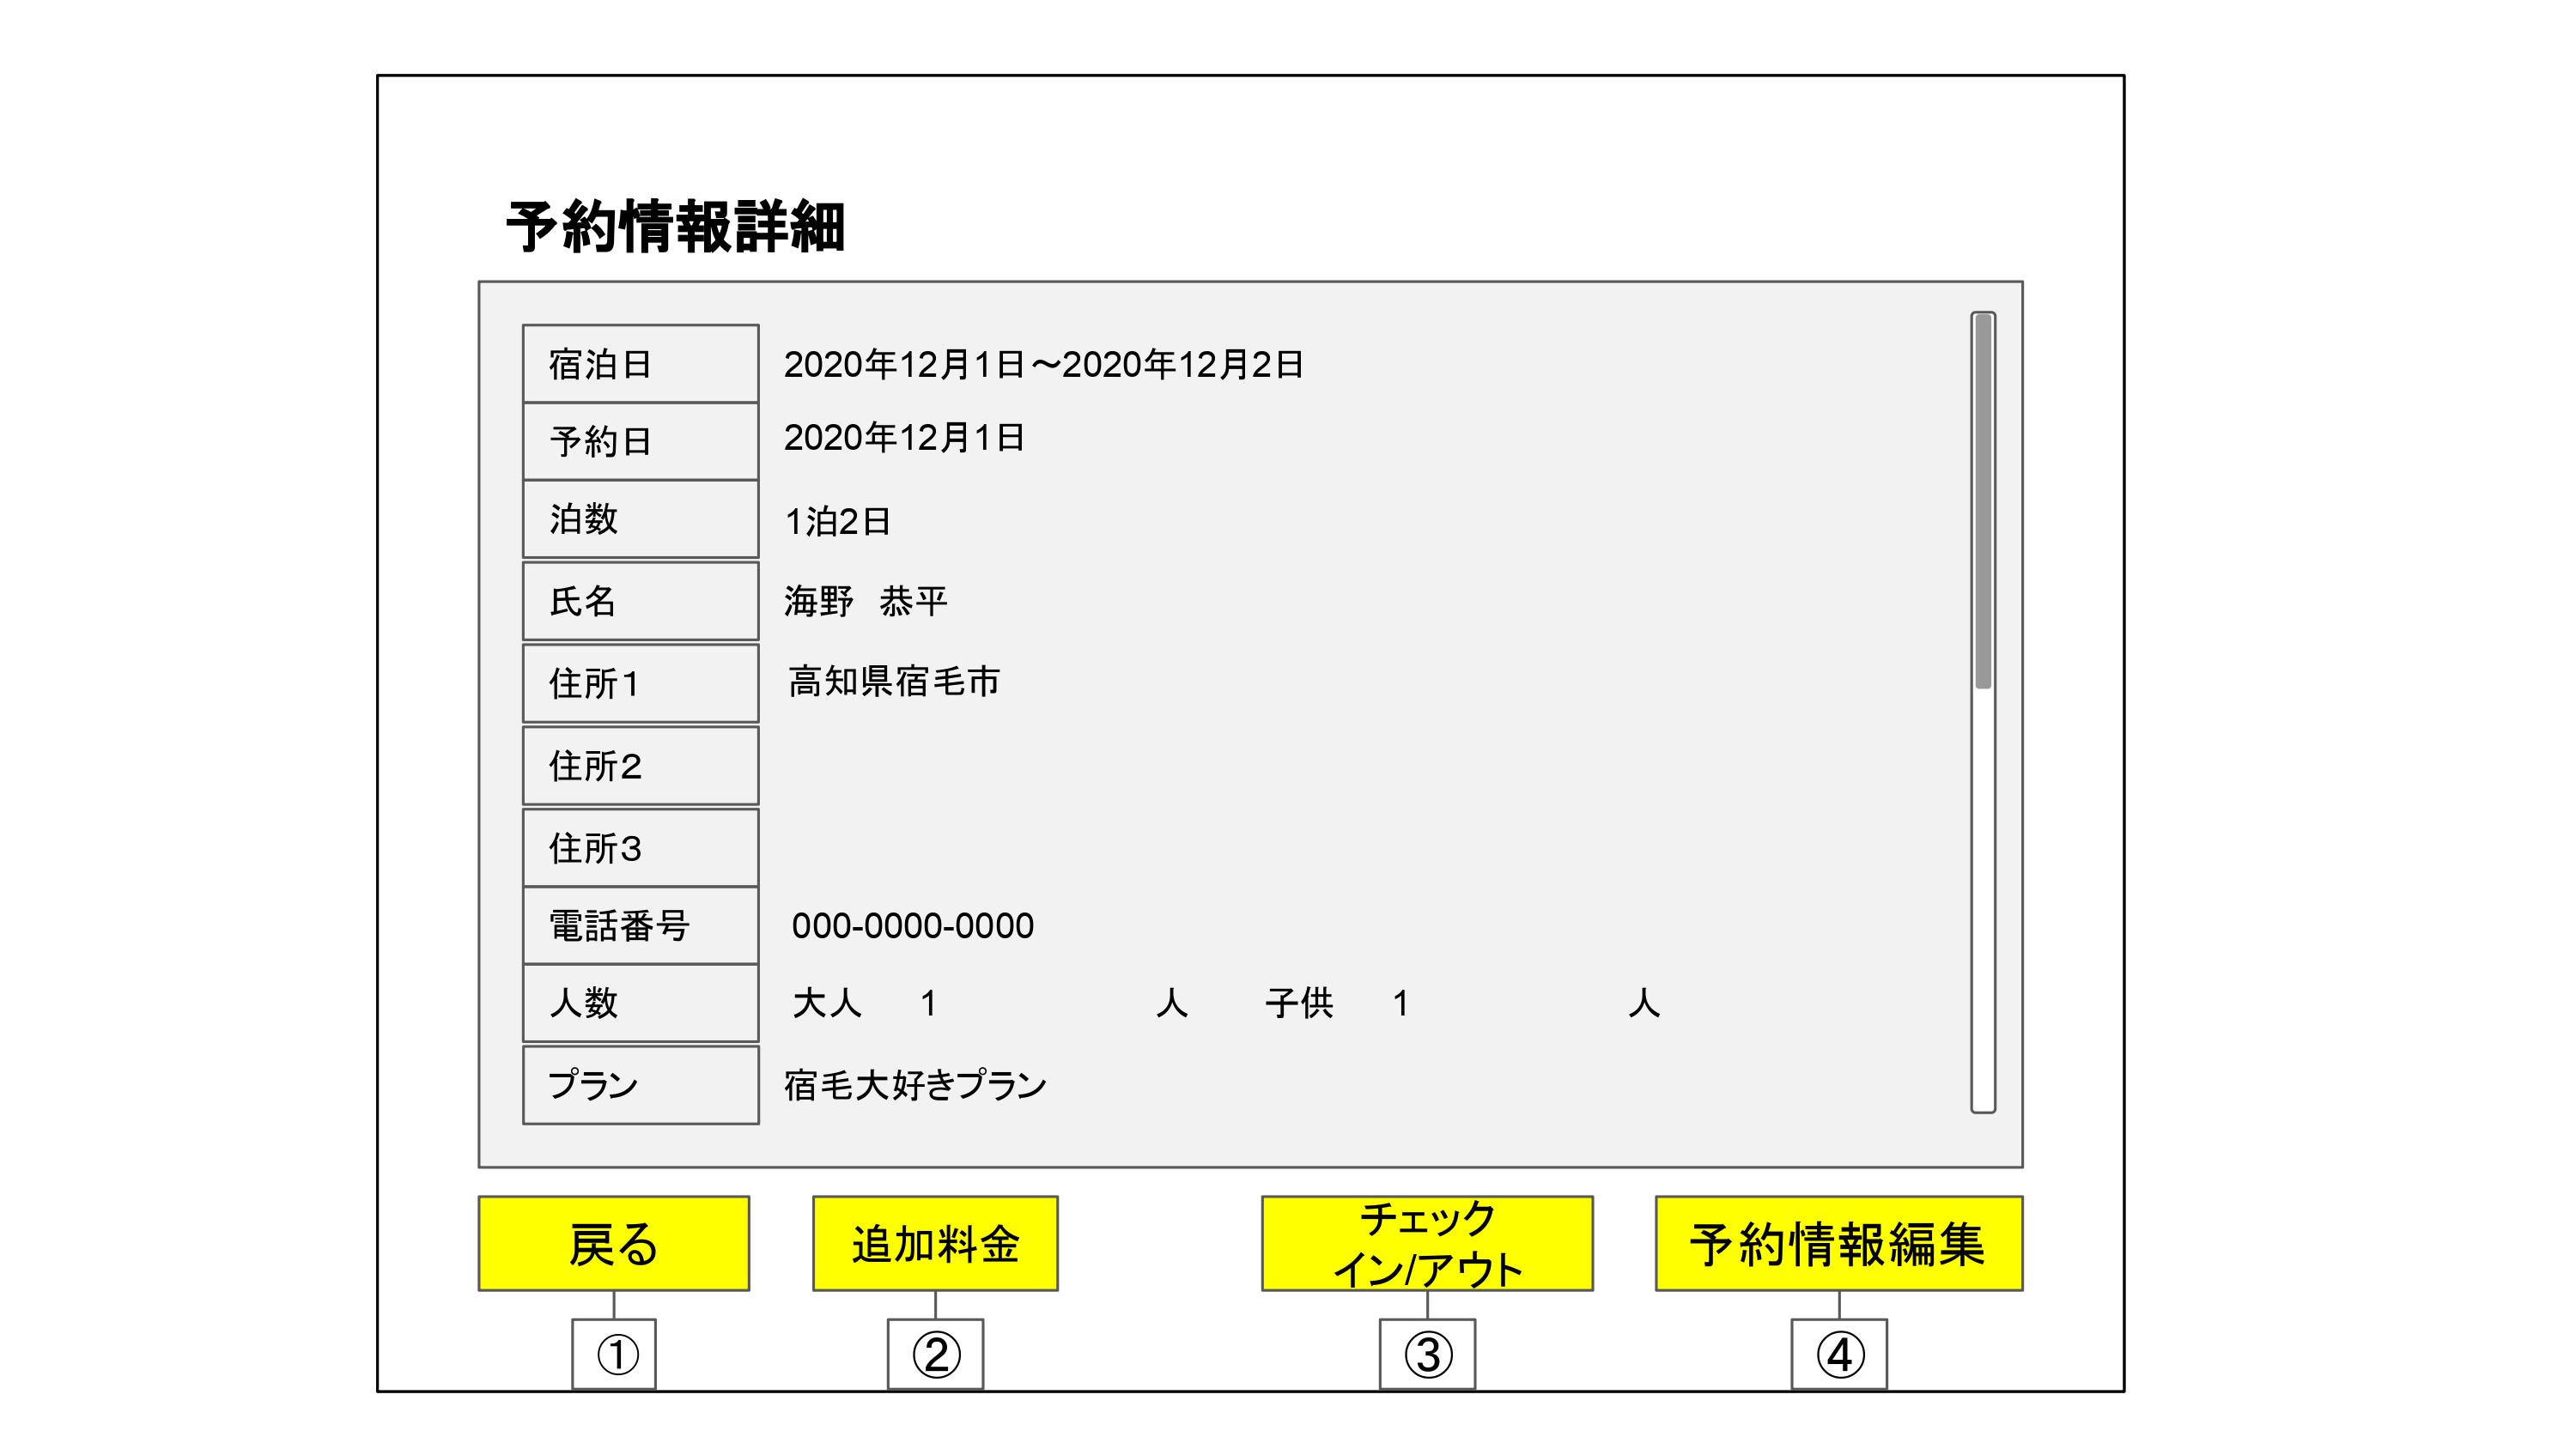
\includegraphics[width=150mm]{UI_front/info1.jpg}
 \caption{予約情報詳細画面1}
 \label{fig:frontinf1}
\end{figure}

\begin{figure}[H]
 \centering
   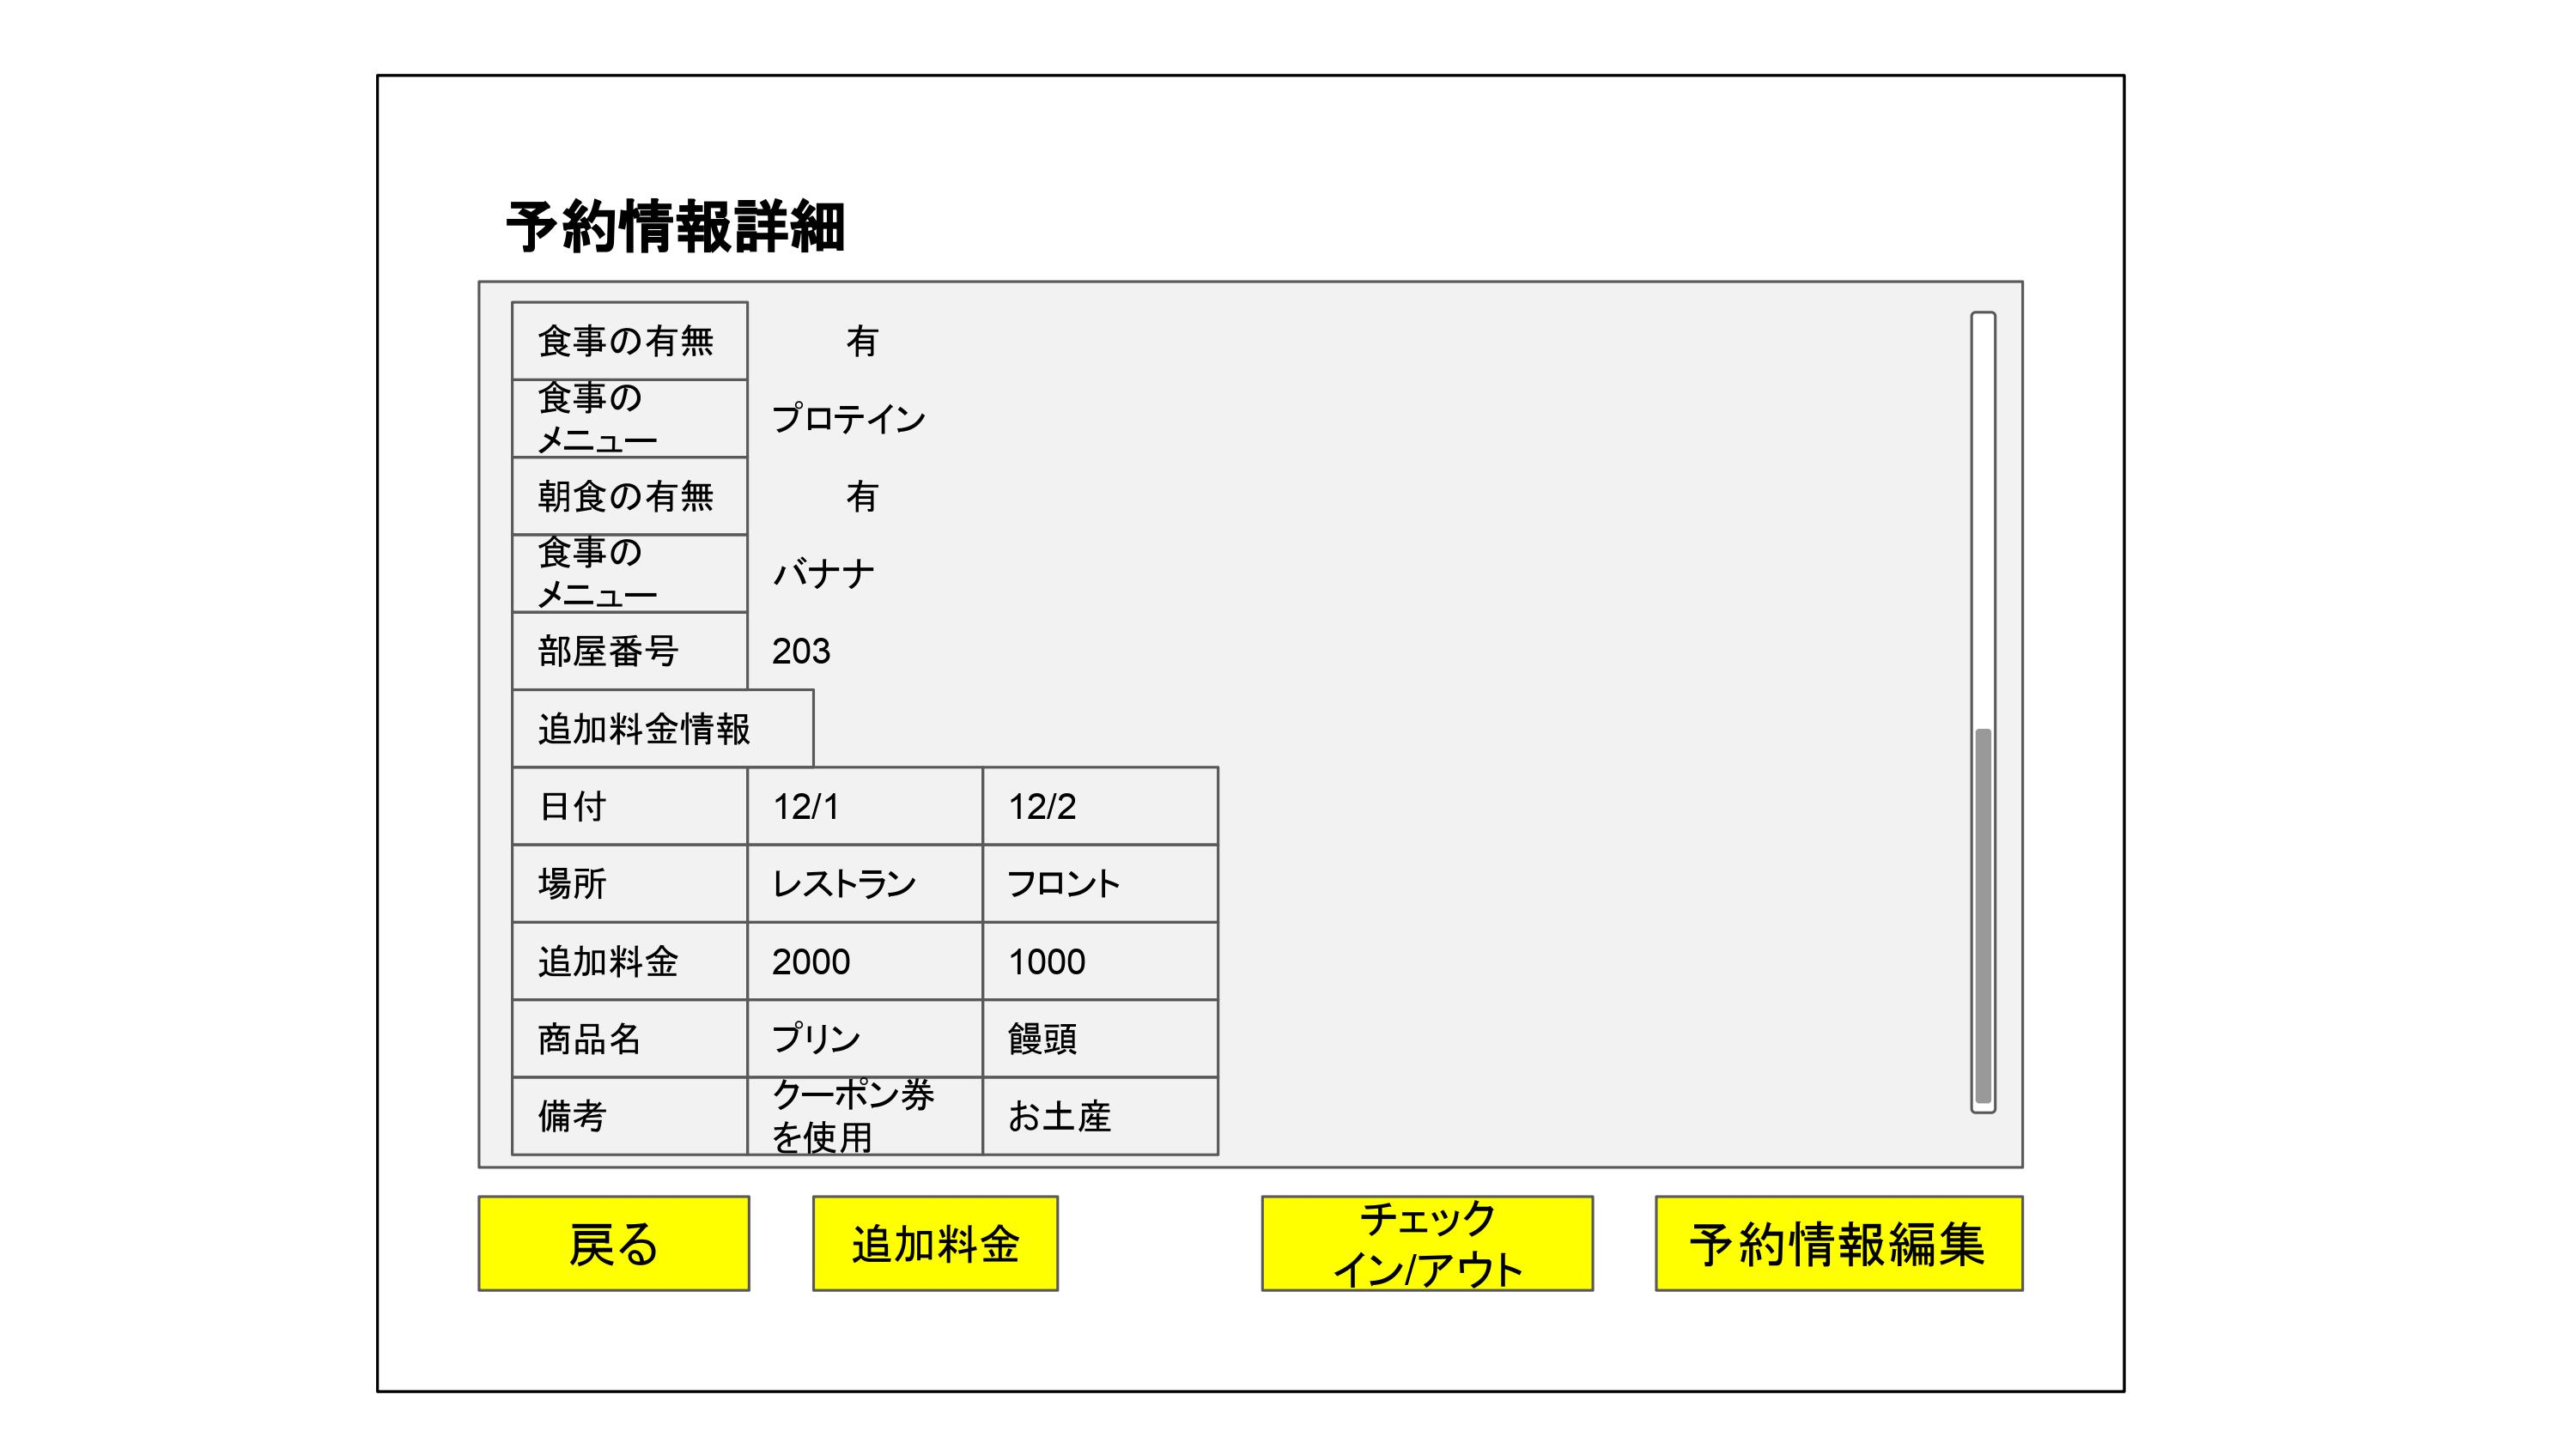
\includegraphics[width=150mm]{UI_front/info2.jpg}
 \caption{予約情報詳細画面2}
 \label{fig:frontinf2}
\end{figure}

\begin{enumerate}
\renewcommand{\labelenumi}{\textcircled{\scriptsize \theenumi}}
\item 戻る\\ 戻るを押すことで,図\ref{fig:frontTop}に示すフロントTOP画面に遷移する.
\item 追加料金\\ 追加料金を押すことで,図\ref{fig:frontF}に示す追加料金編集画面に遷移する.
\item チェックイン/アウト\\ チェックインしている場合は,チェックアウトを表示する.
\item 予約情報編集\\ 予約情報編集を押すことで,図\ref{fig:frontR1},図\ref{fig:frontR2}に示す予約情報編集画面に遷移する.
\end{enumerate}

\subsubsection{予約入力画面}
 図\ref{fig:frontR1},図\ref{fig:frontR2}に予約入力画面を示す.

\begin{figure}[H]
 \centering
   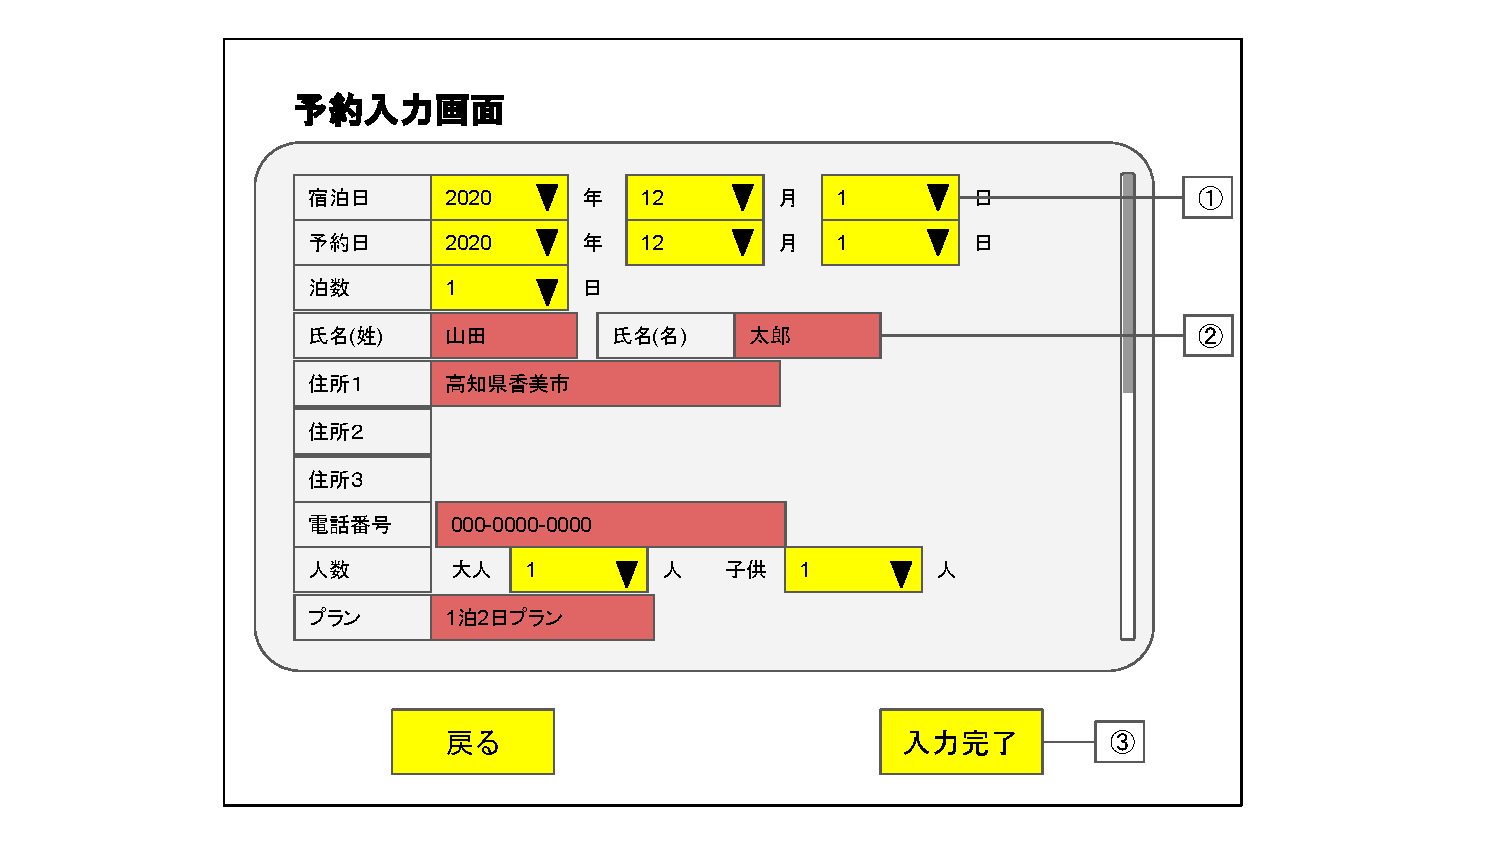
\includegraphics[width=150mm]{UI_front/Input-Reservation-screen.pdf}
 \caption{予約入力画面1}
 \label{fig:frontR1}
\end{figure}
\begin{figure}[H]
 \centering
   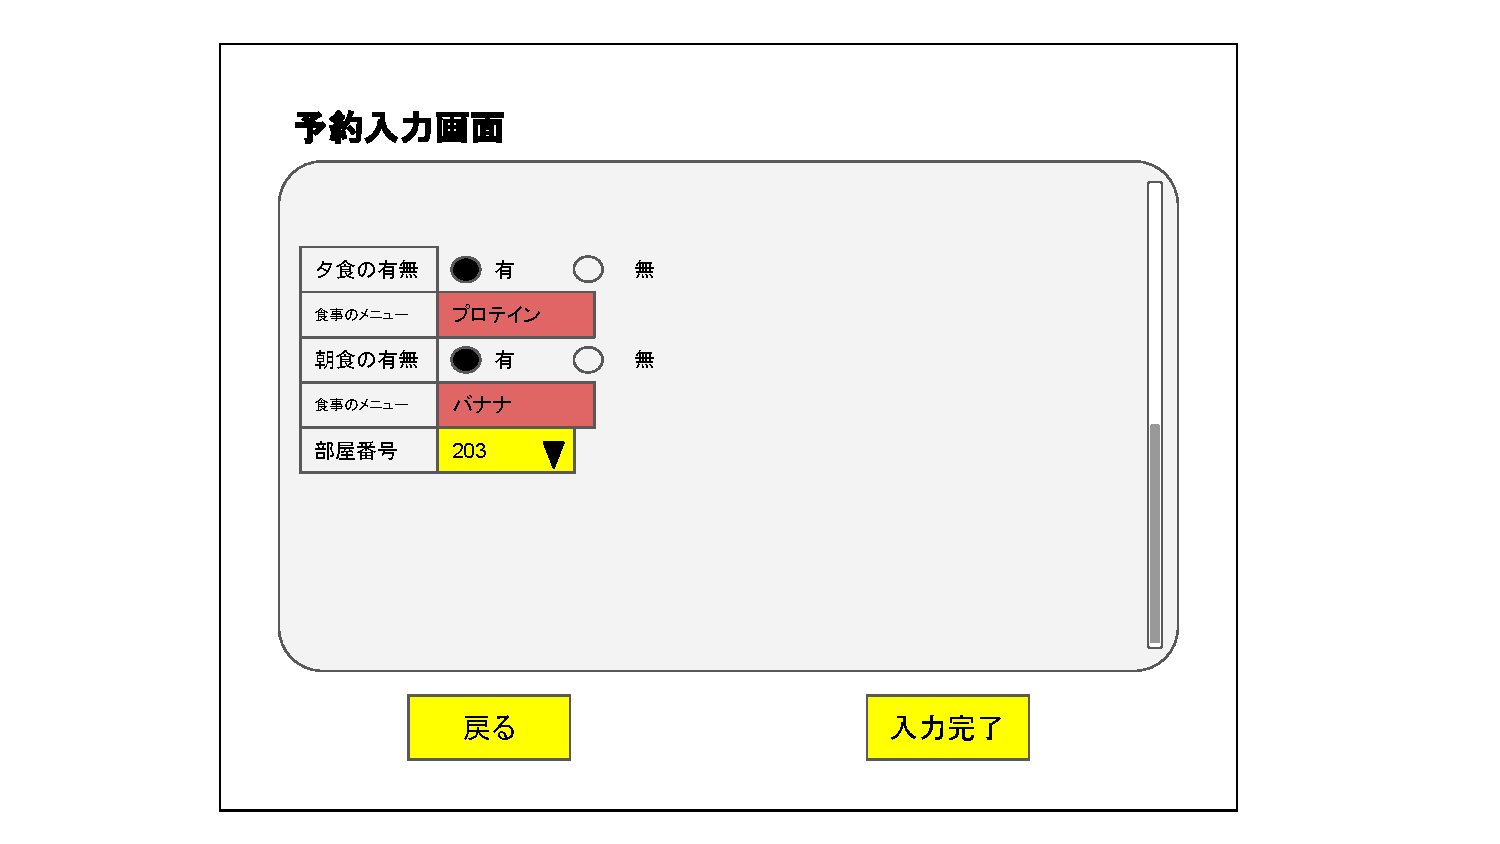
\includegraphics[width=150mm]{UI_front/Input-Reservation-screen02.pdf}
 \caption{予約入力画面2}
 \label{fig:frontR2}
\end{figure}


\begin{figure}[H]
 \centering
   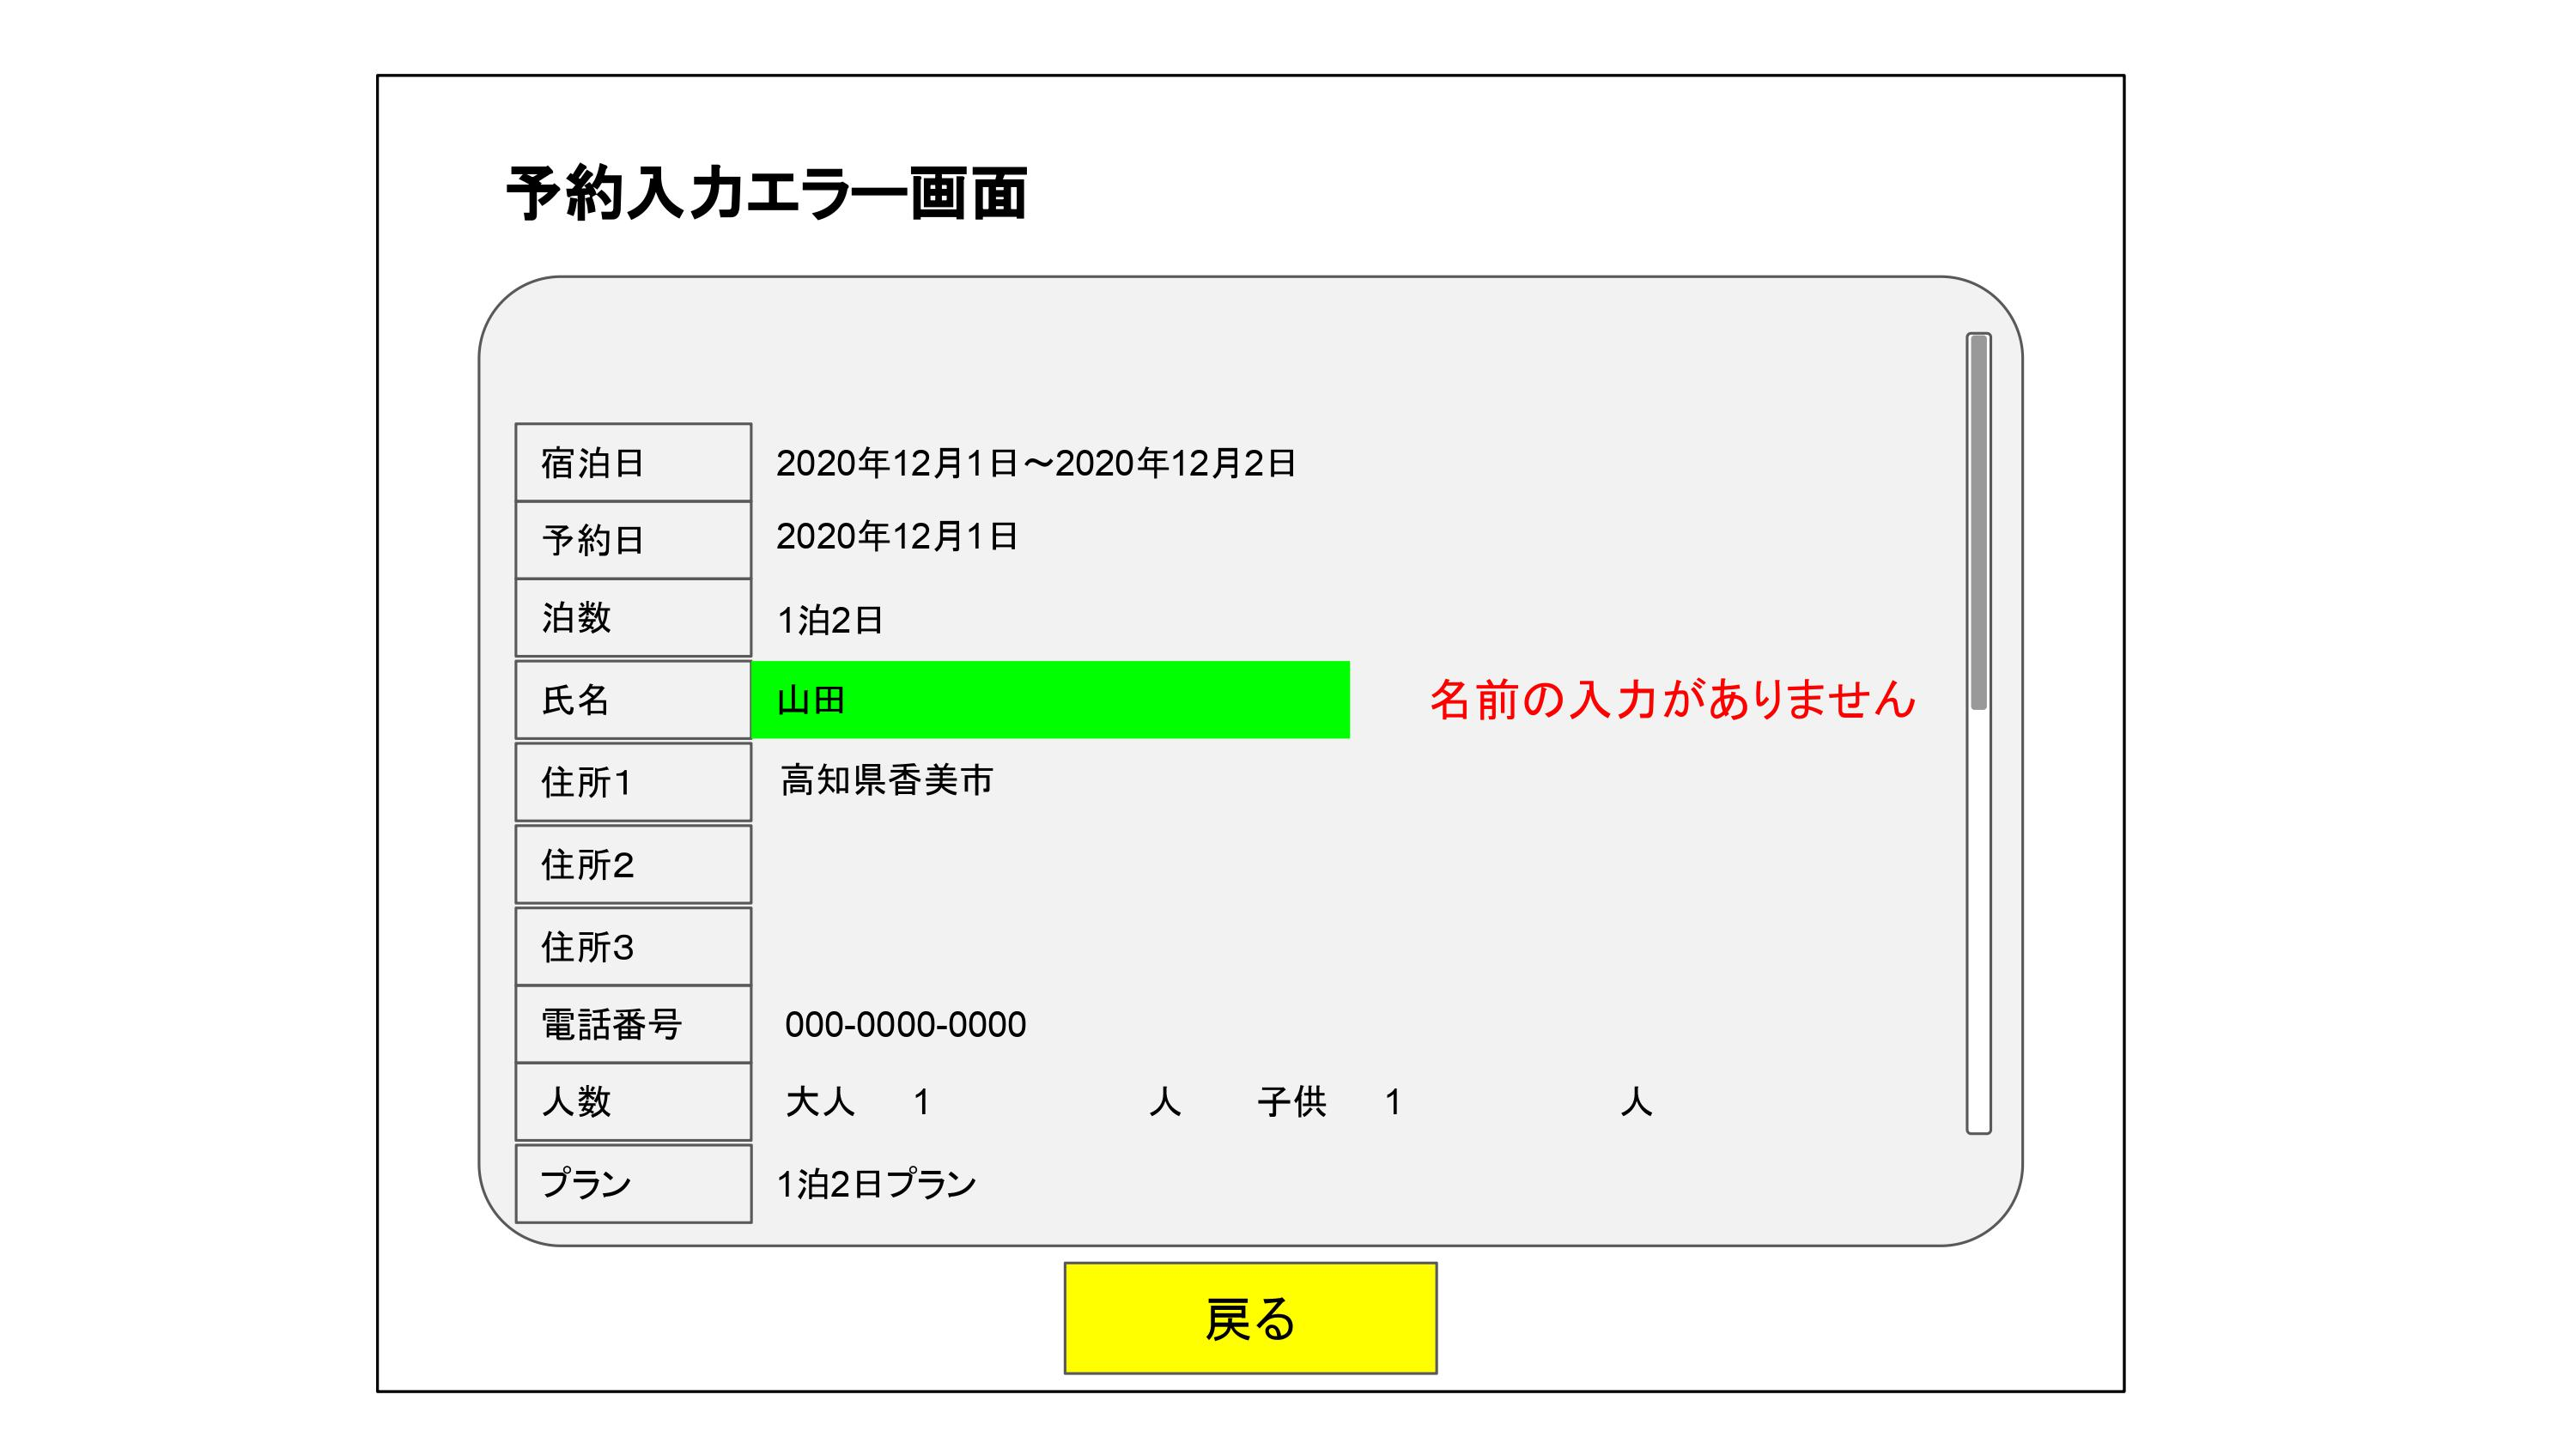
\includegraphics[width=150mm]{UI_front/reseE1.jpg}
 \caption{予約入力エラー画面1}
 \label{fig:frontRE1}
\end{figure}
\begin{figure}[H]
 \centering
   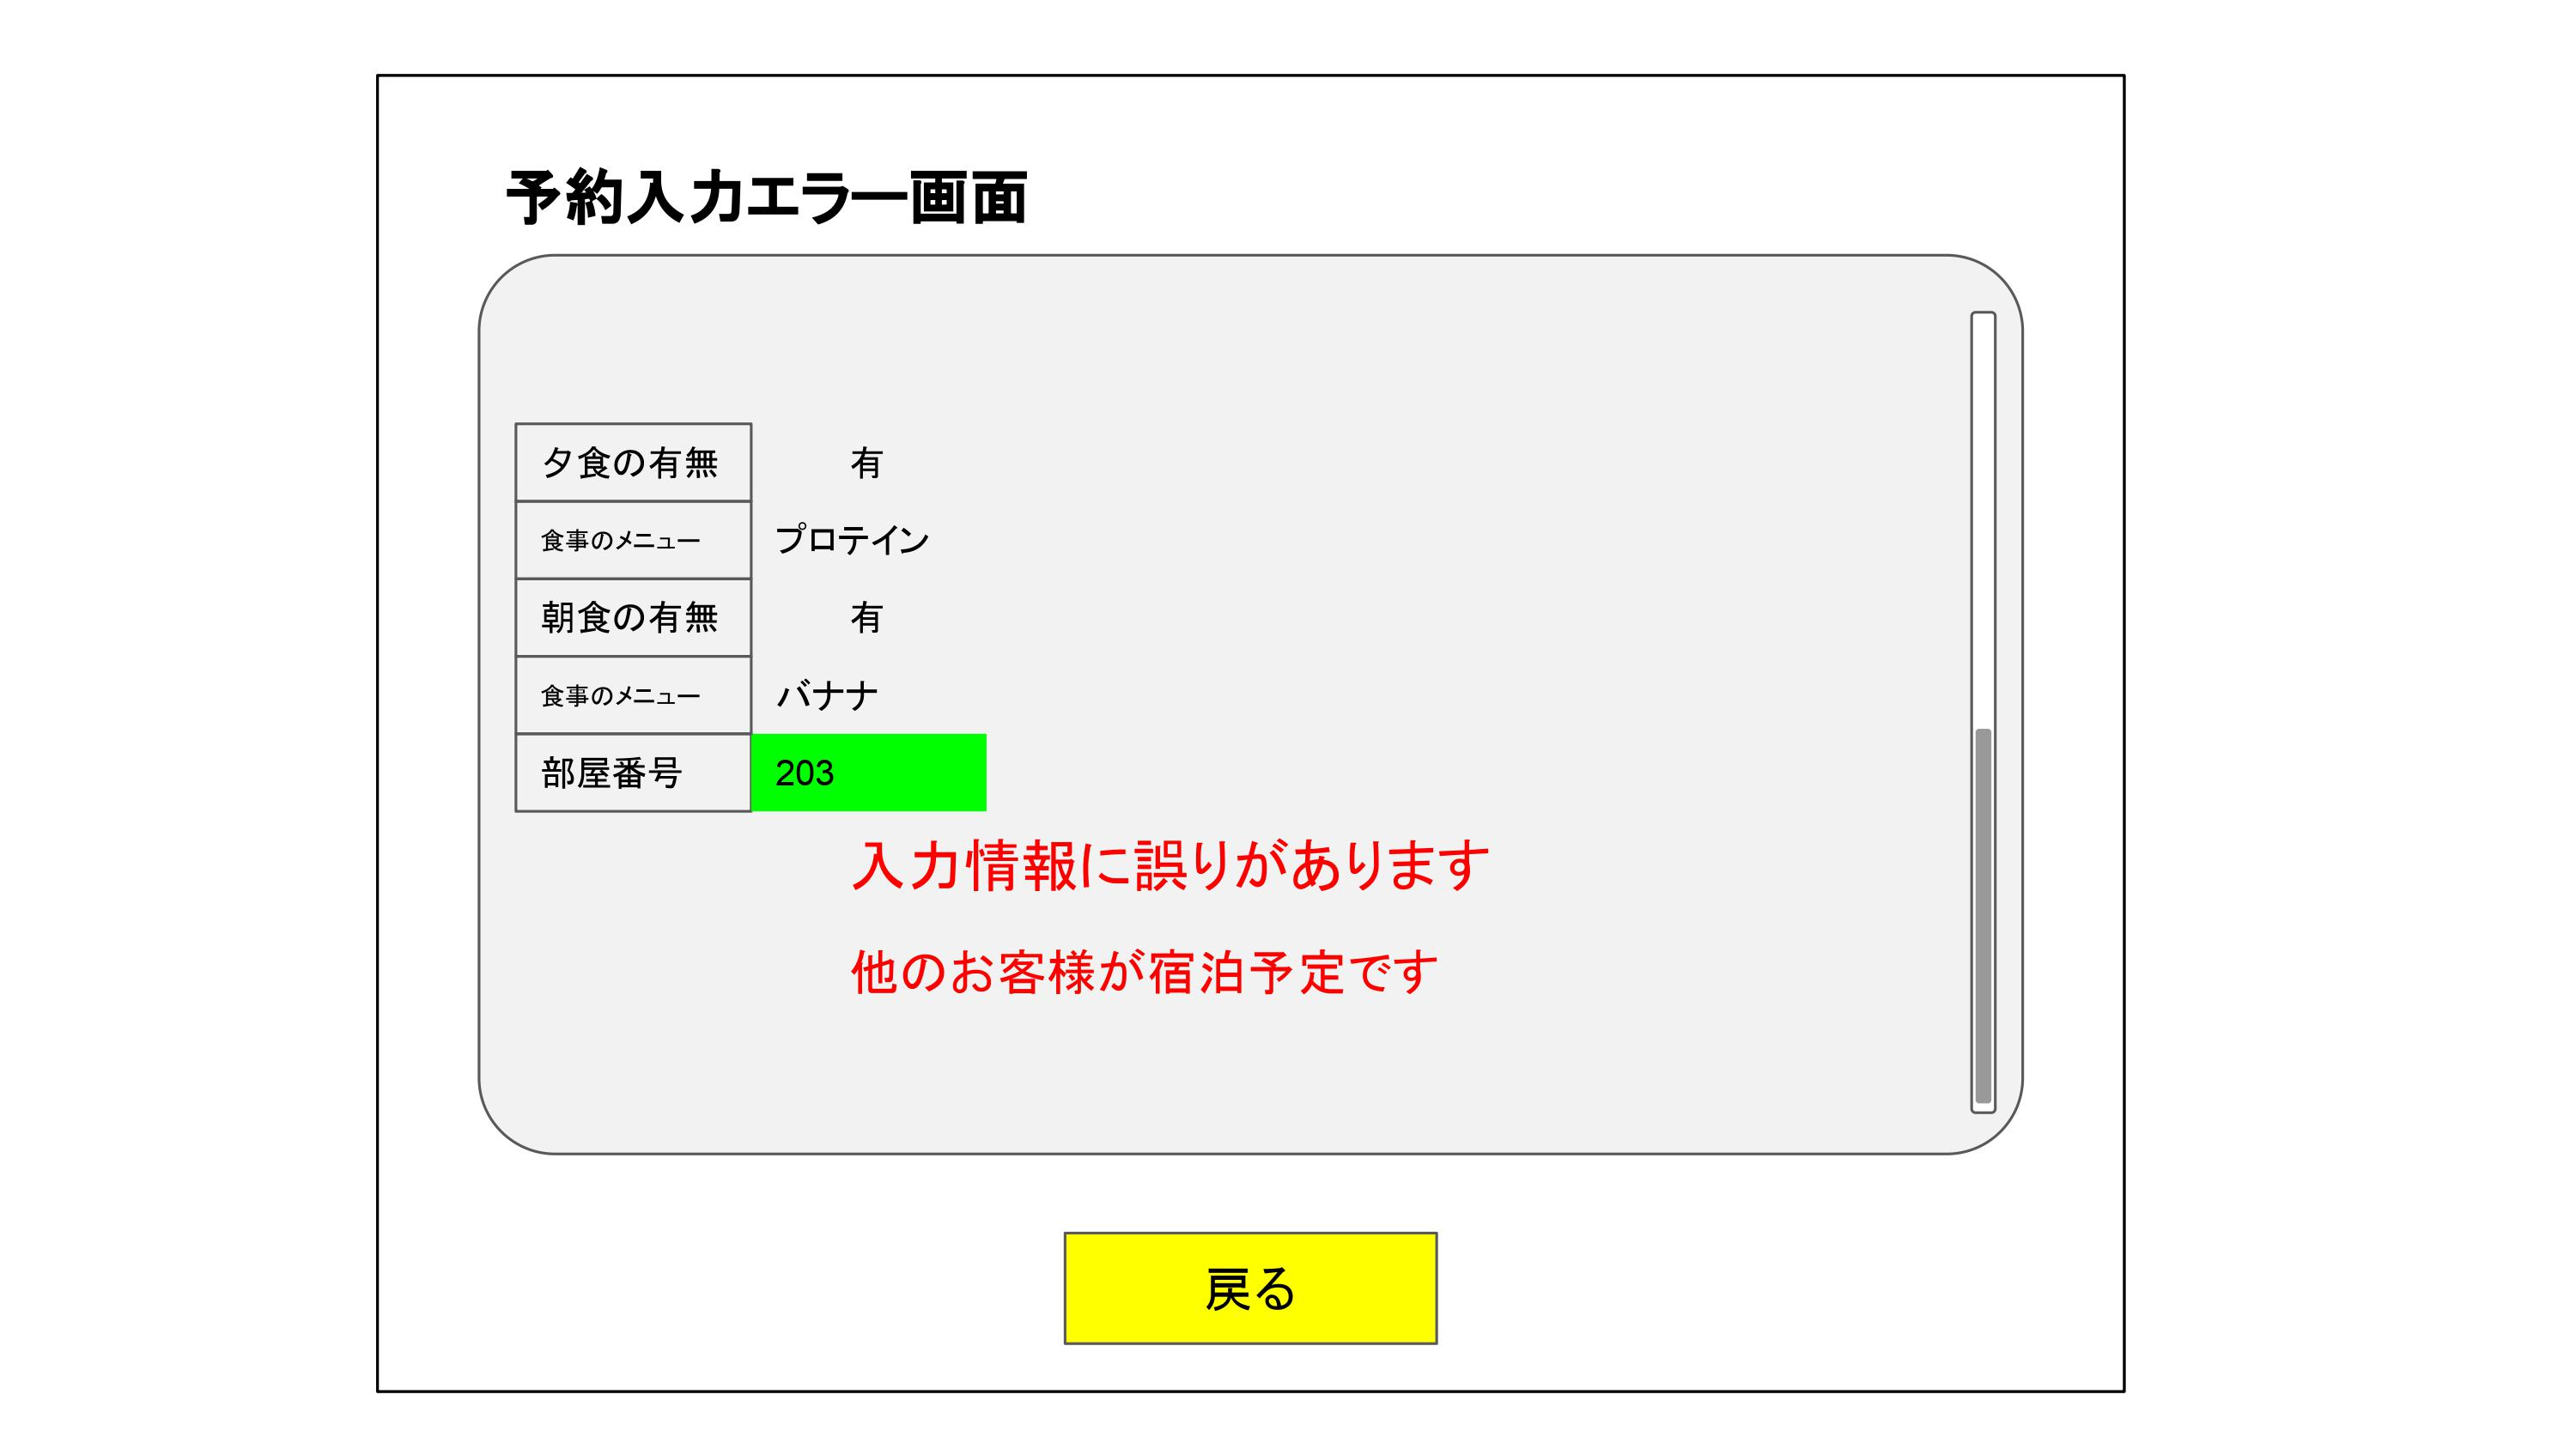
\includegraphics[width=150mm]{UI_front/reseE2.jpg}
 \caption{予約入力エラー画面2}
 \label{fig:frontRE2}
\end{figure}


\begin{enumerate}
\renewcommand{\labelenumi}{\textcircled{\scriptsize \theenumi}}
\item 日付,人数の選択\\ ドロップダウンリストを押すことで,日付,人数を選択する.
\item 記入欄\\ 赤の欄を押すことで,キーボード入力を行う.
\item 入力完了\\ 入力完了を押すことで,図\ref{fig:frontRe1},図\ref{fig:frontRe2}に示す入力確認画面に遷移する.入力に不足や誤りがある場合は,図\ref{fig:frontRE1},図\ref{fig:frontRE2}に示す予約入力エラーメッセージを表示する.
\end{enumerate}


\subsubsection{予約入力確認画面}
 図\ref{fig:frontRe1},図\ref{fig:frontRe2}に予約入力確認画面を示す.

\begin{figure}[H]
 \centering
   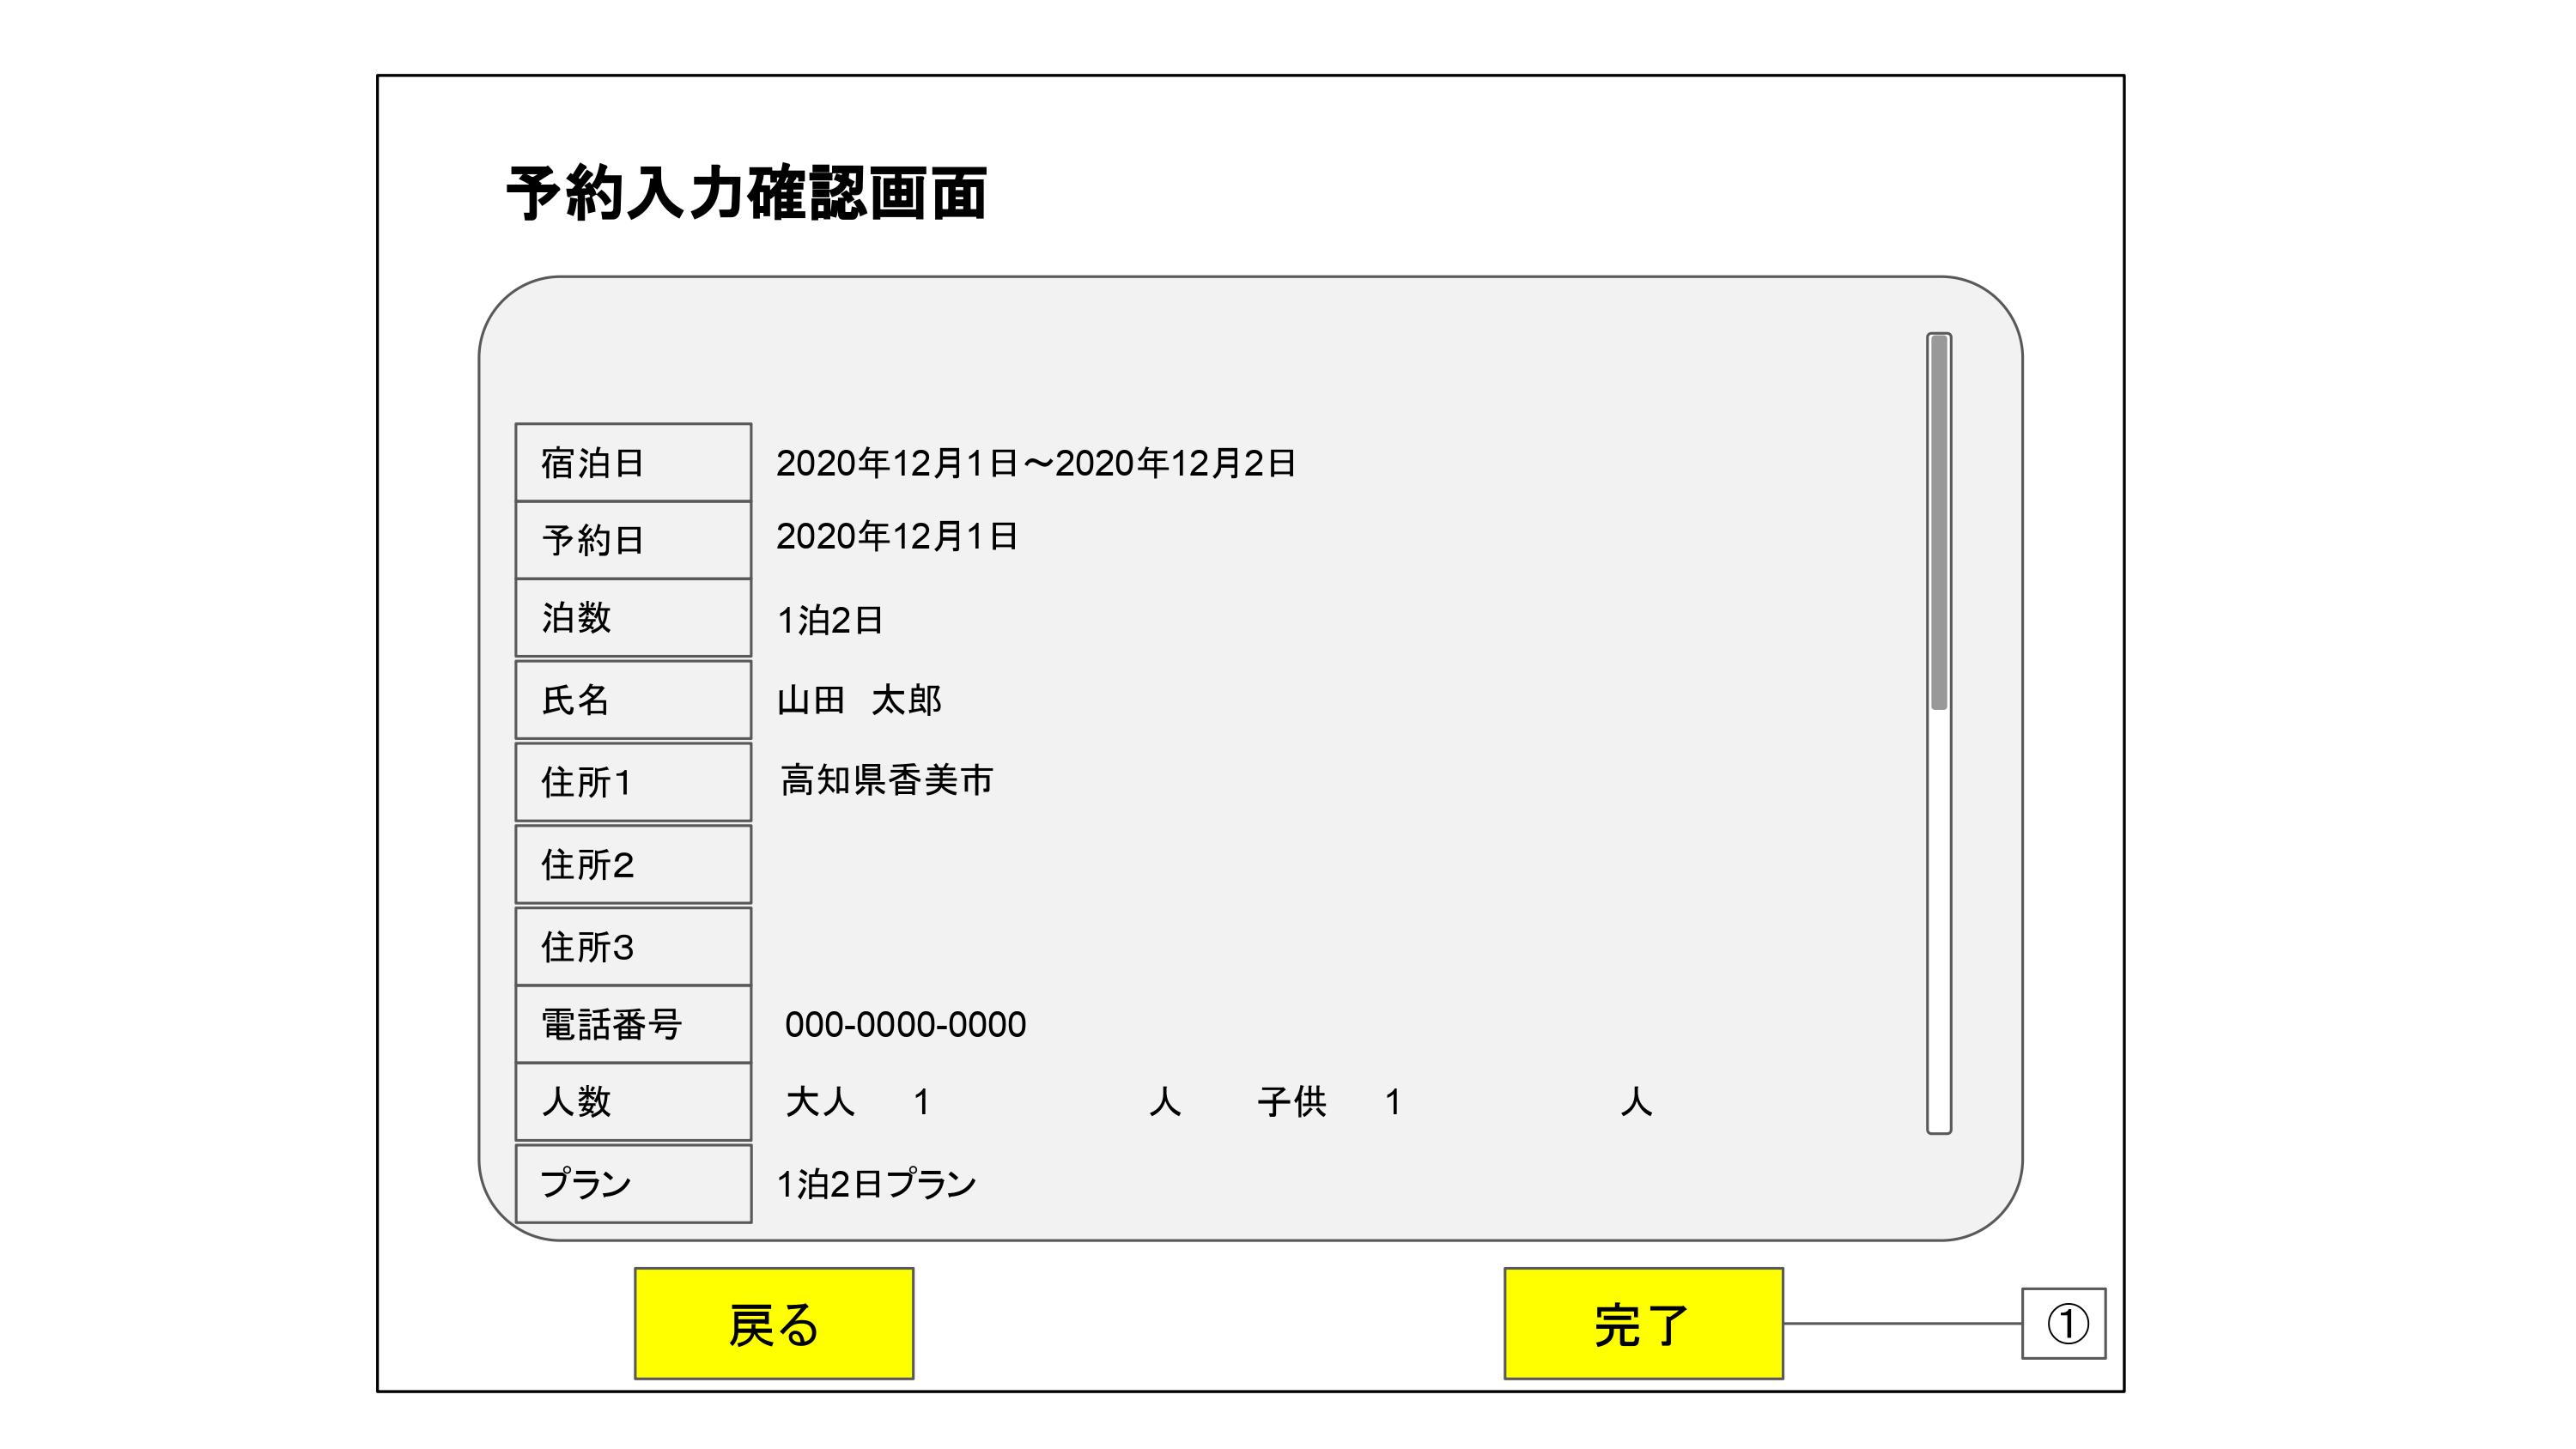
\includegraphics[width=150mm]{UI_front/reseC1.jpg}
 \caption{予約入力確認画面1}
 \label{fig:frontRe1}
\end{figure}

\begin{figure}[H]
 \centering
   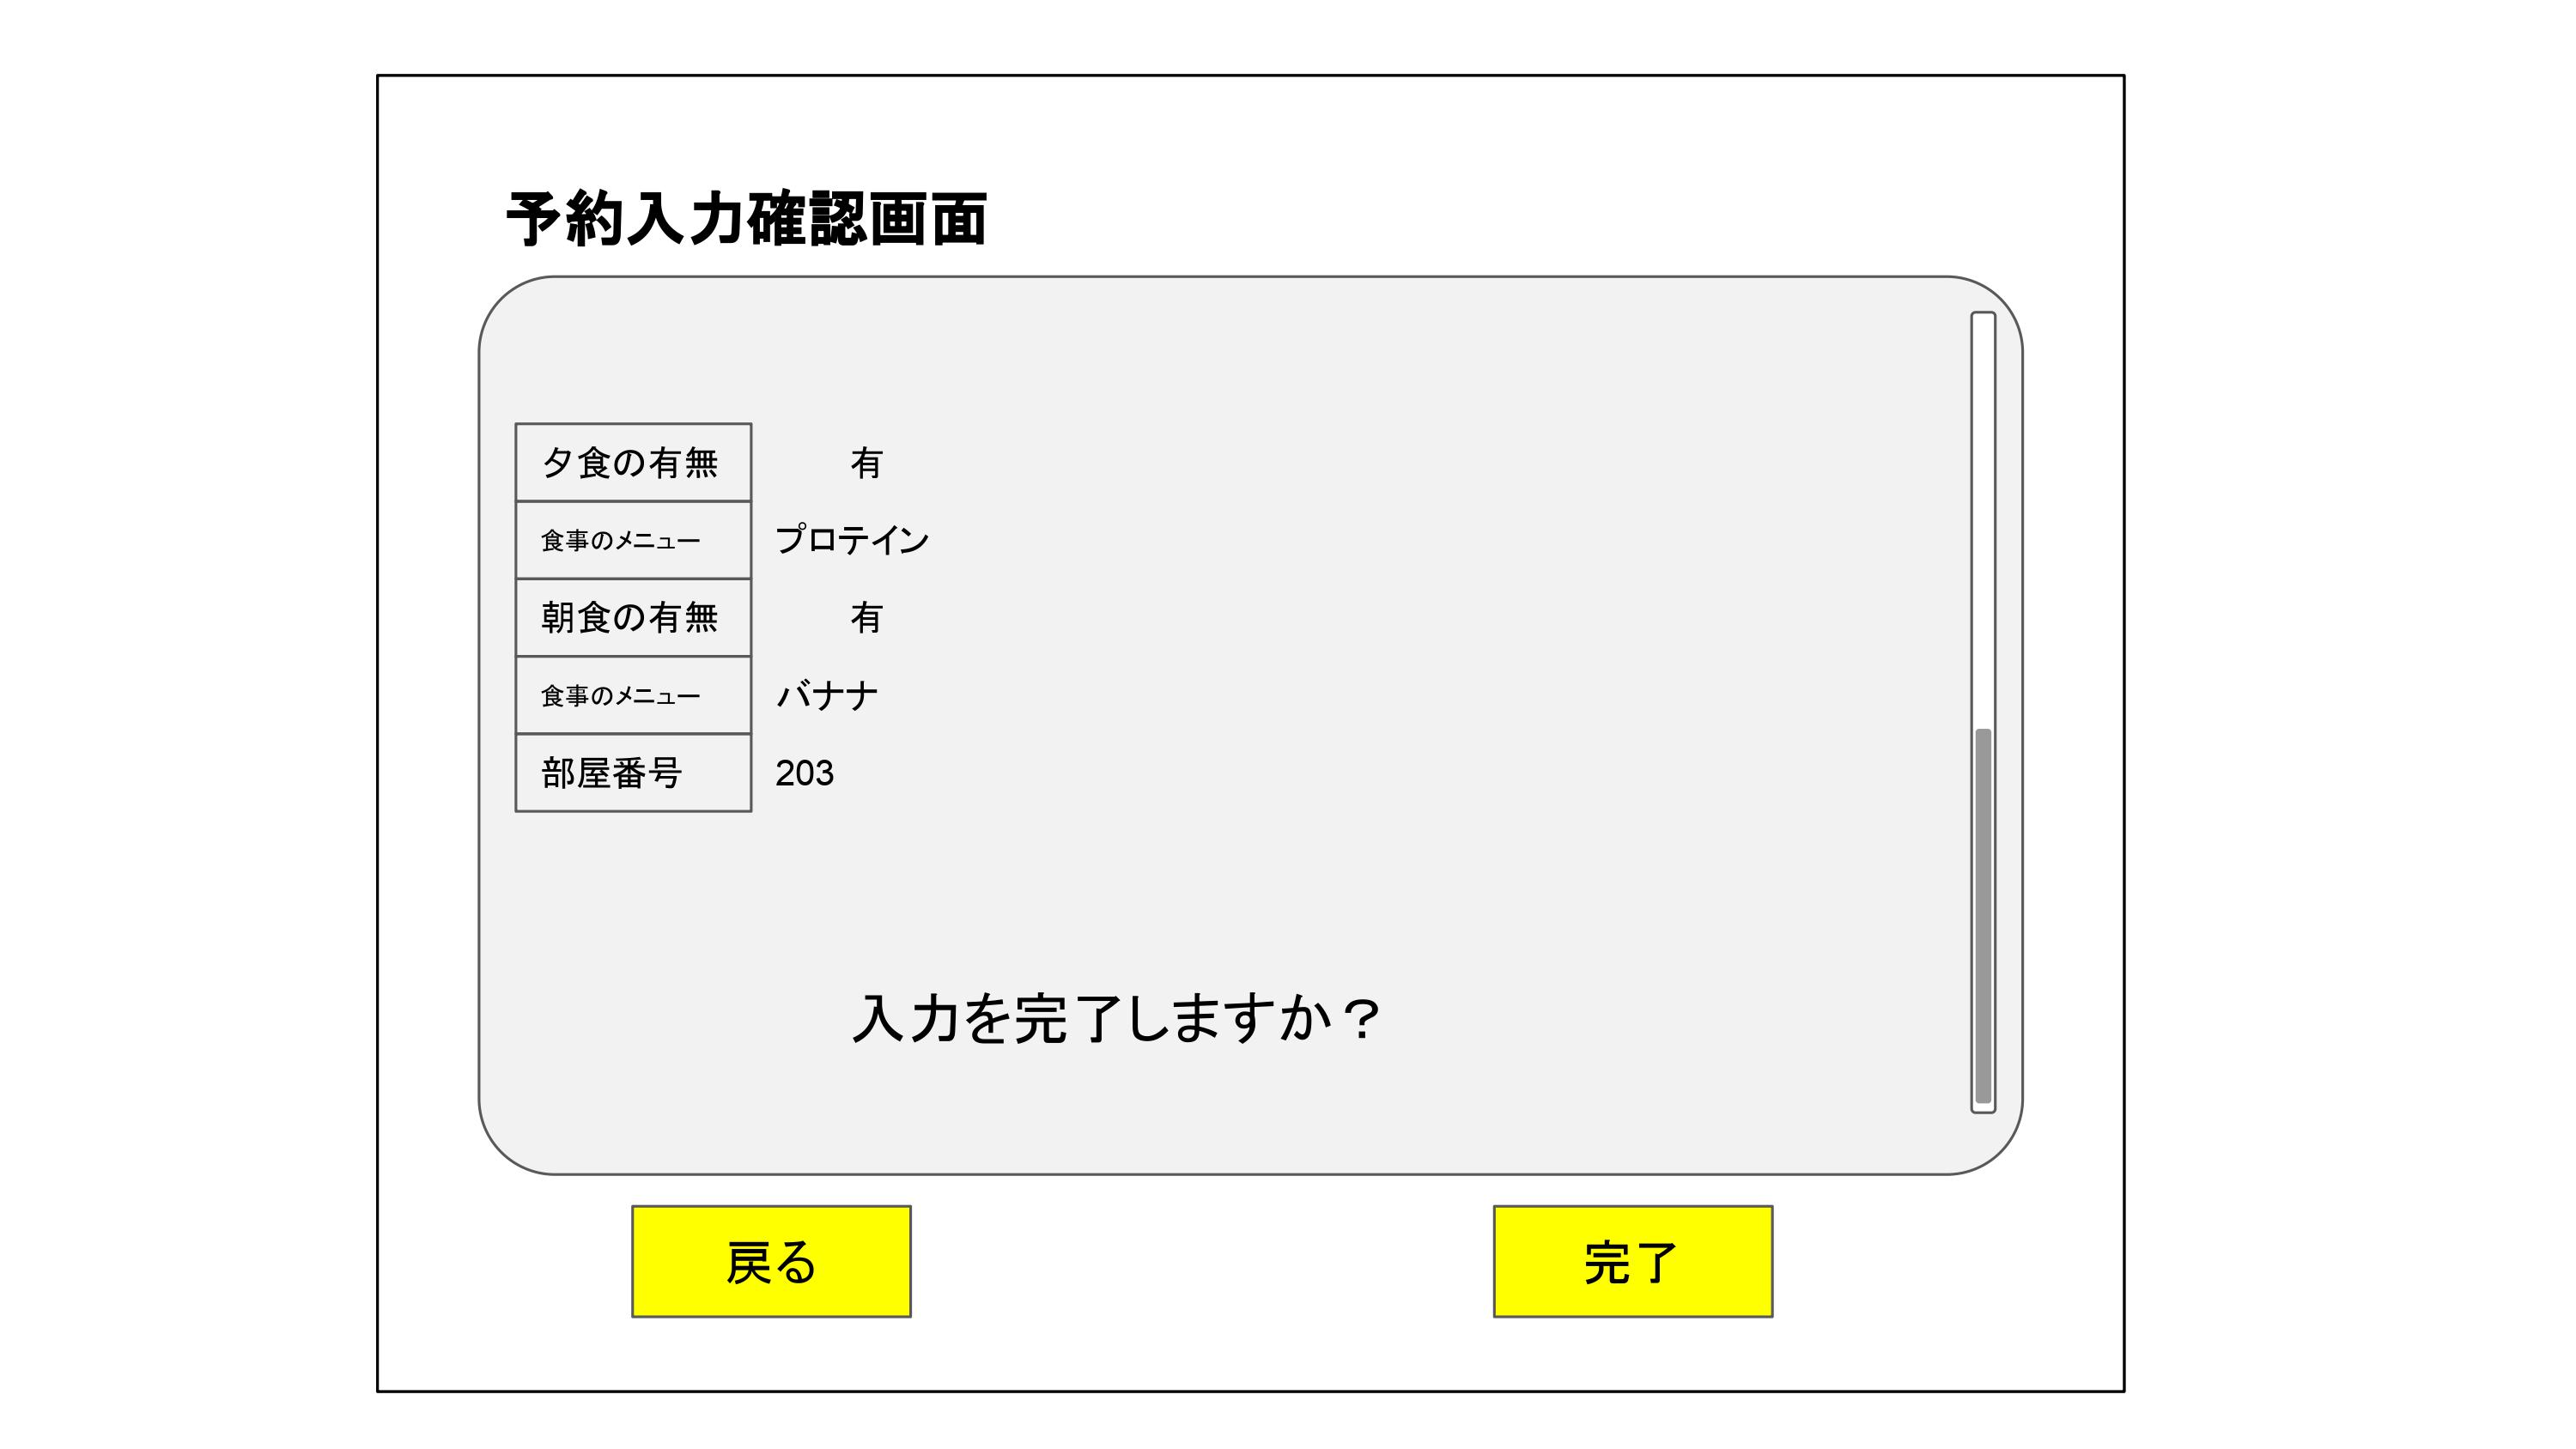
\includegraphics[width=150mm]{UI_front/reseC2.jpg}
 \caption{予約入力確認画面2}
 \label{fig:frontRe2}
\end{figure}


\begin{enumerate}
\renewcommand{\labelenumi}{\textcircled{\scriptsize \theenumi}}
\item 完了\\ 完了を押すことで,図\ref{fig:frontRc}に示す入力完了画面に遷移する.
\end{enumerate}


\subsubsection{予約入力完了画面}
 図\ref{fig:frontRc}に予約入力完了画面を示す.

\begin{figure}[H]
 \centering
   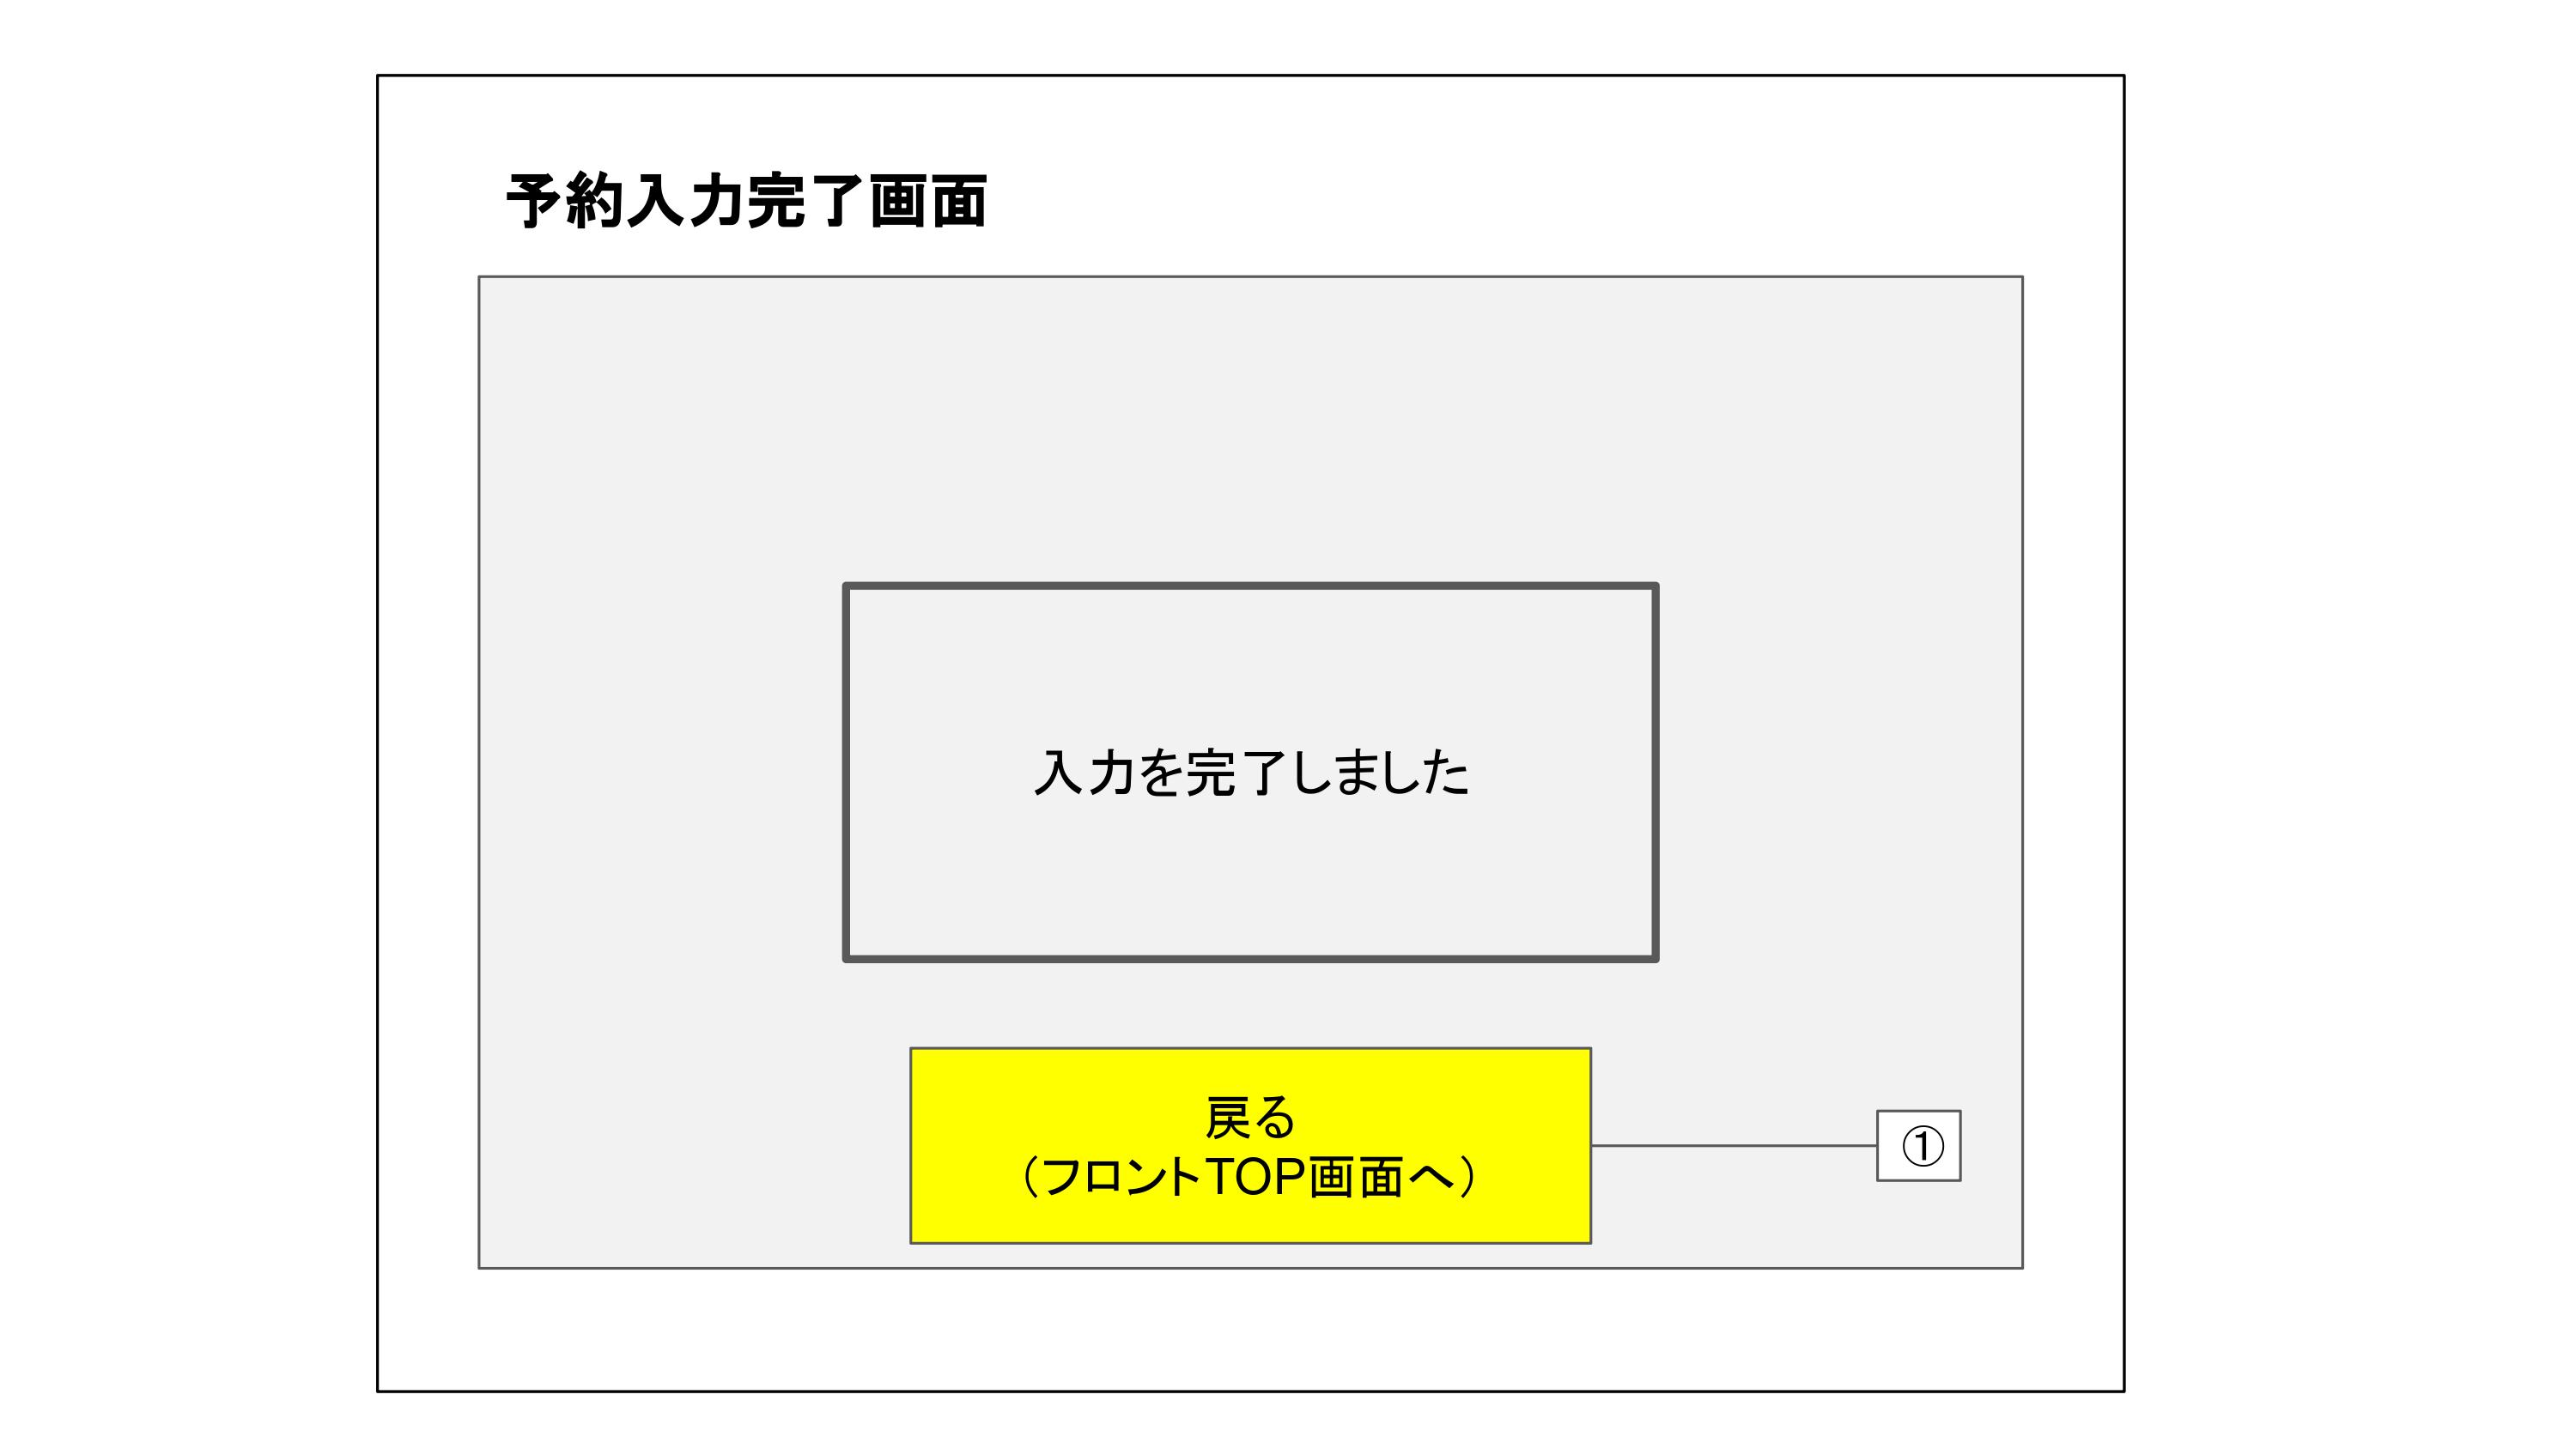
\includegraphics[width=150mm]{UI_front/reseD.jpg}
 \caption{予約入力完了画面}
 \label{fig:frontRc}
\end{figure}


\begin{enumerate}
\renewcommand{\labelenumi}{\textcircled{\scriptsize \theenumi}}
\item 戻る\\ 戻るを押すことで,図\ref{fig:frontTop}に示すフロントTOP画面に遷移する.
\end{enumerate}


\subsubsection{追加料金編集画面}
 図\ref{fig:frontF}に追加料金編集画面を示す.

\begin{figure}[H]
 \centering
   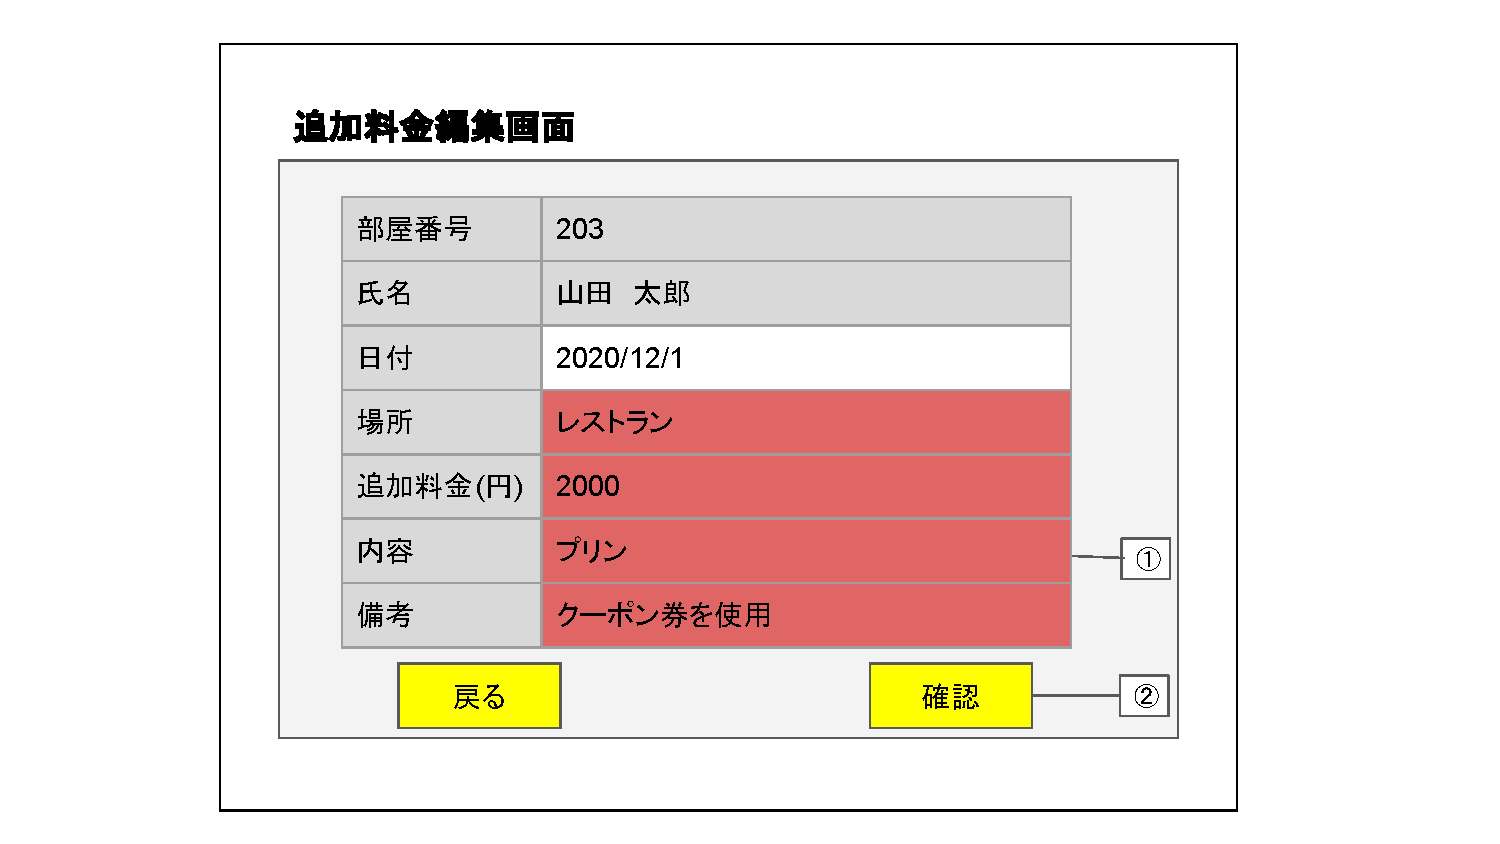
\includegraphics[width=150mm]{UI_front/Additional-Fee-screen.pdf}
 \caption{追加料金編集画面}
 \label{fig:frontF}
\end{figure}


\begin{enumerate}
\renewcommand{\labelenumi}{\textcircled{\scriptsize \theenumi}}
%\item 場所の選択\\ ドロップダウンリストを押すことで,レストランかフロントの選択をする.
\item 場所,料金,メニュー,備考\\ 赤の欄を押すことで,場所,追加料金,メニュー,備考を入力する.
\item 確認\\ 確認を押すことで,図\ref{fig:frontFe}に示す追加料金確認画面に遷移する.
\end{enumerate}


\subsubsection{追加料金確認画面}
 図\ref{fig:frontFe}に追加料金確認画面を示す.

\begin{figure}[H]
 \centering
   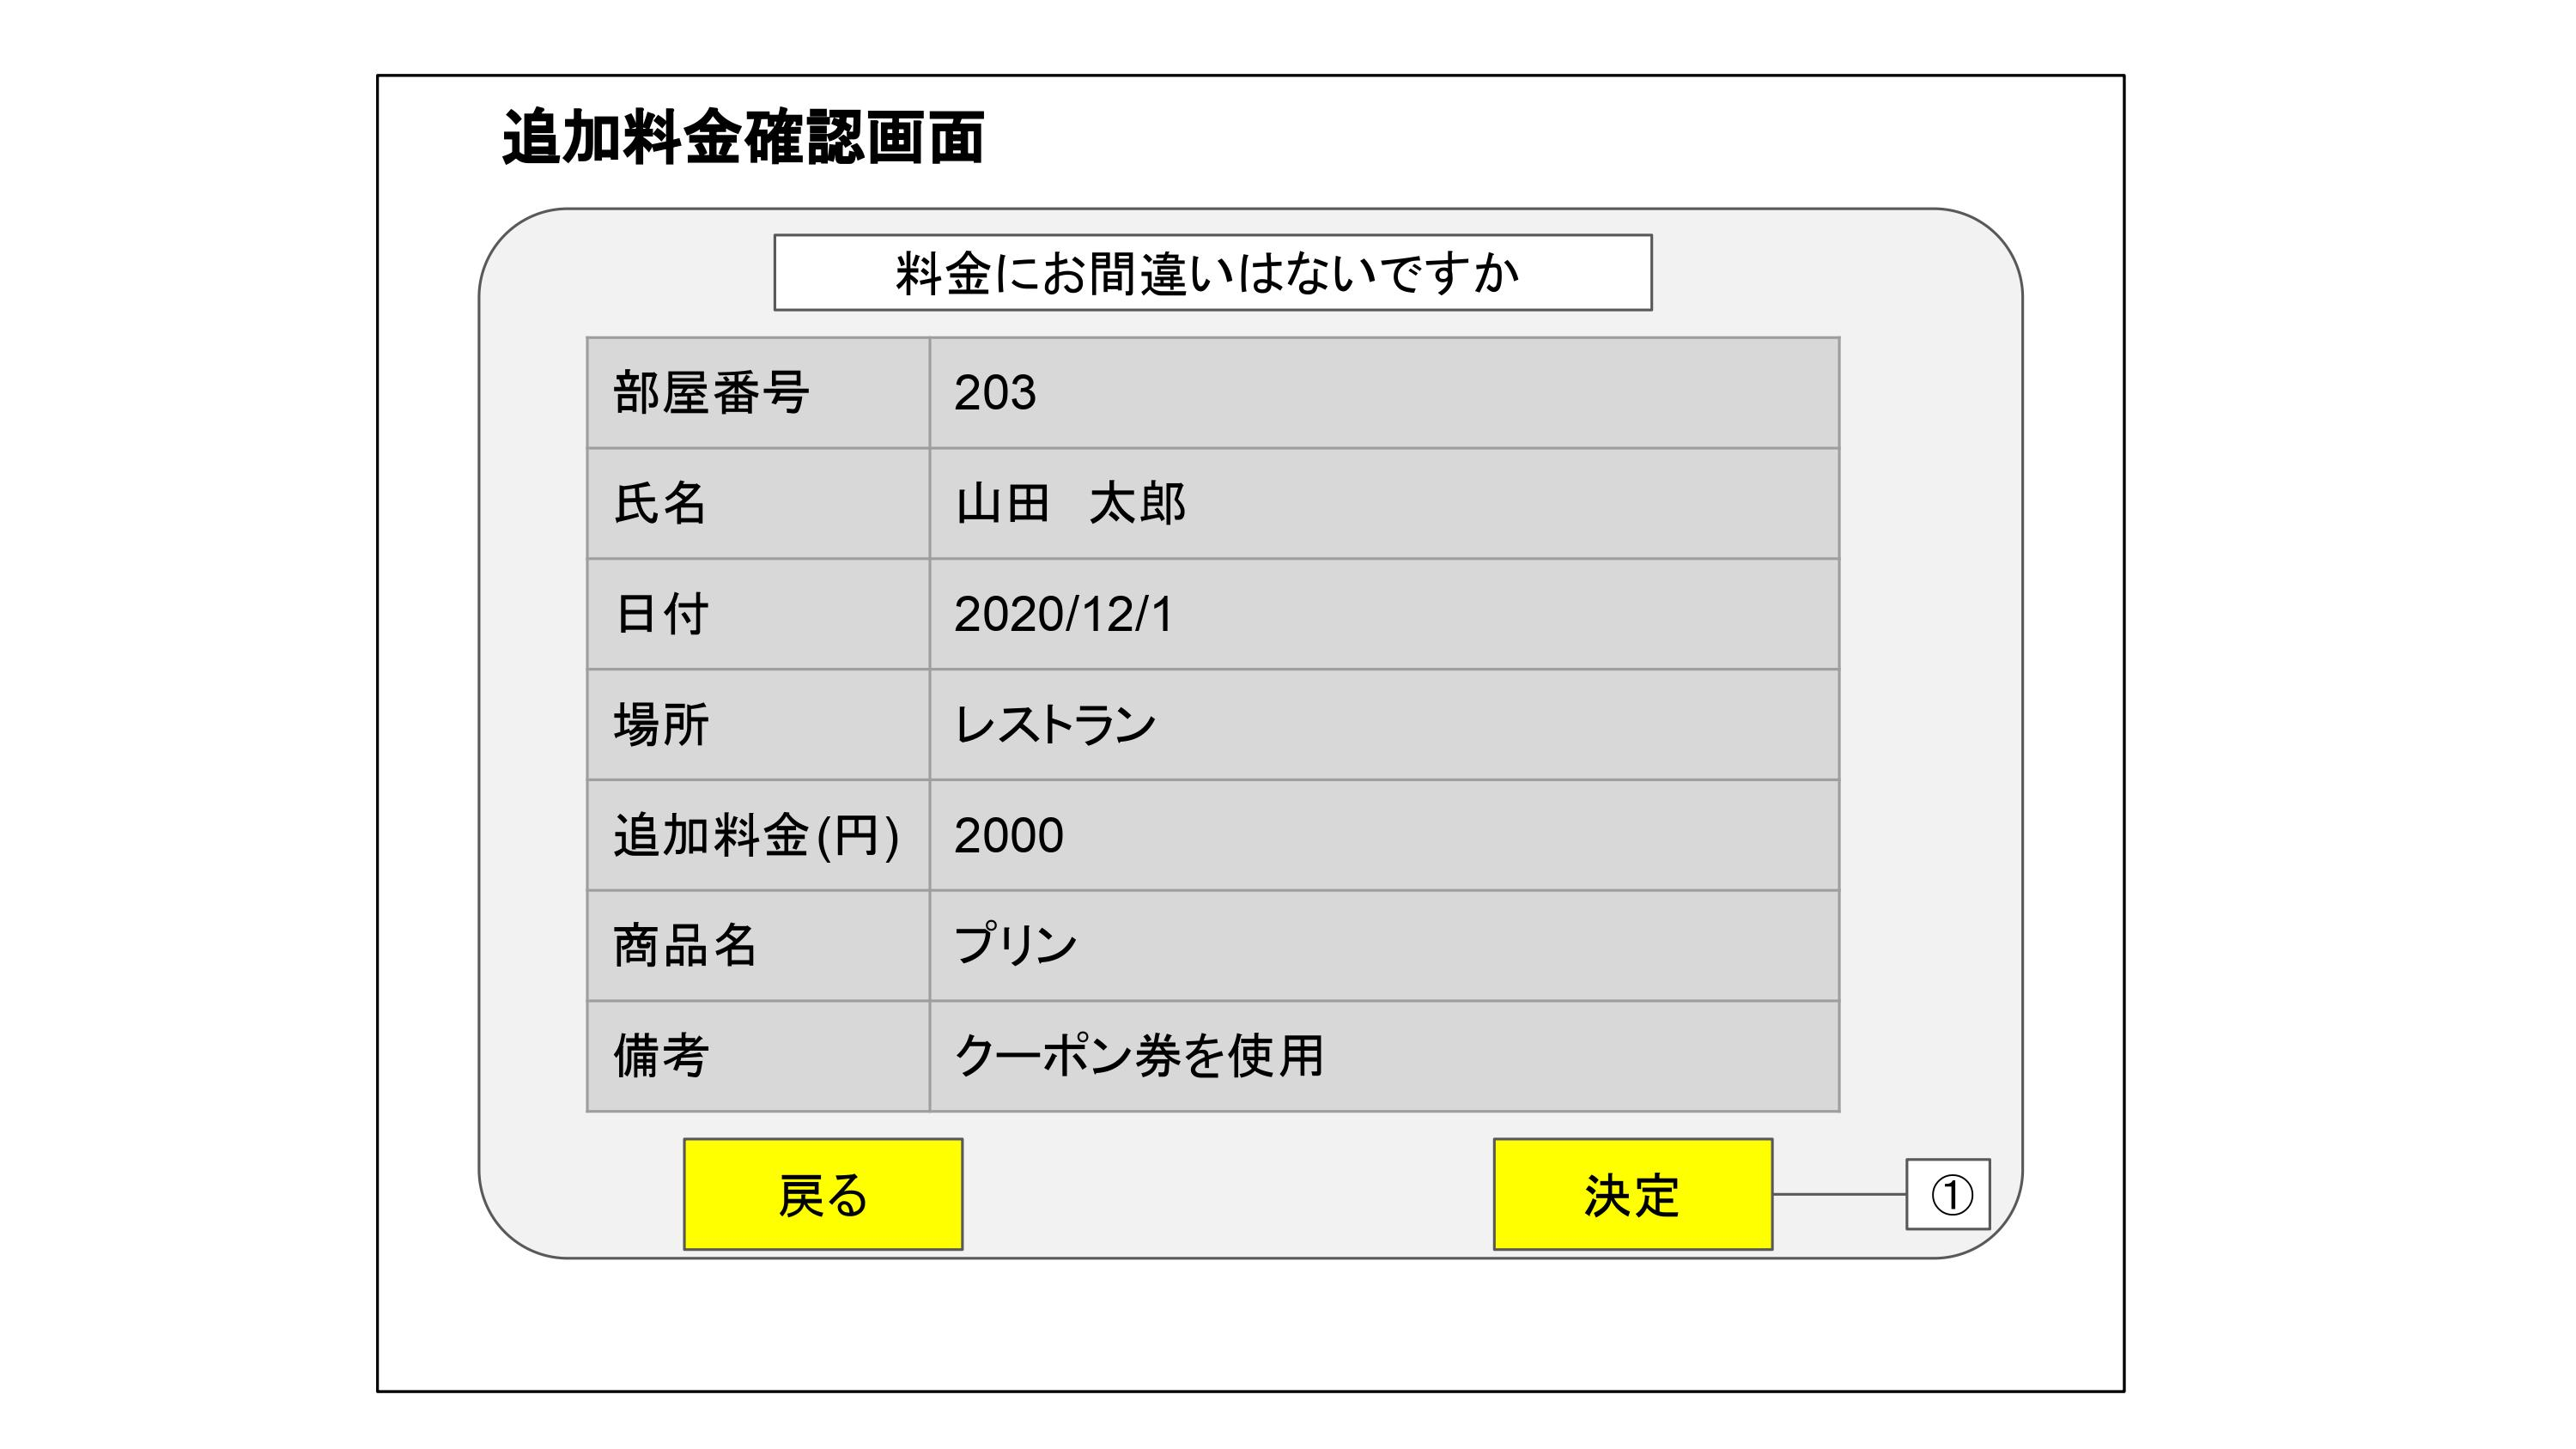
\includegraphics[width=150mm]{UI_front/addfC.jpg}
 \caption{追加料金確認画面}
 \label{fig:frontFe}
\end{figure}

\begin{enumerate}
\renewcommand{\labelenumi}{\textcircled{\scriptsize \theenumi}}
\item 決定\\ 決定を押すことで,図\ref{fig:frontFc}に示す追加料金完了画面に遷移する.
\end{enumerate}


\subsubsection{追加料金完了画面}
 図\ref{fig:frontFc}に追加料金完了画面を示す.

\begin{figure}[H]
 \centering
   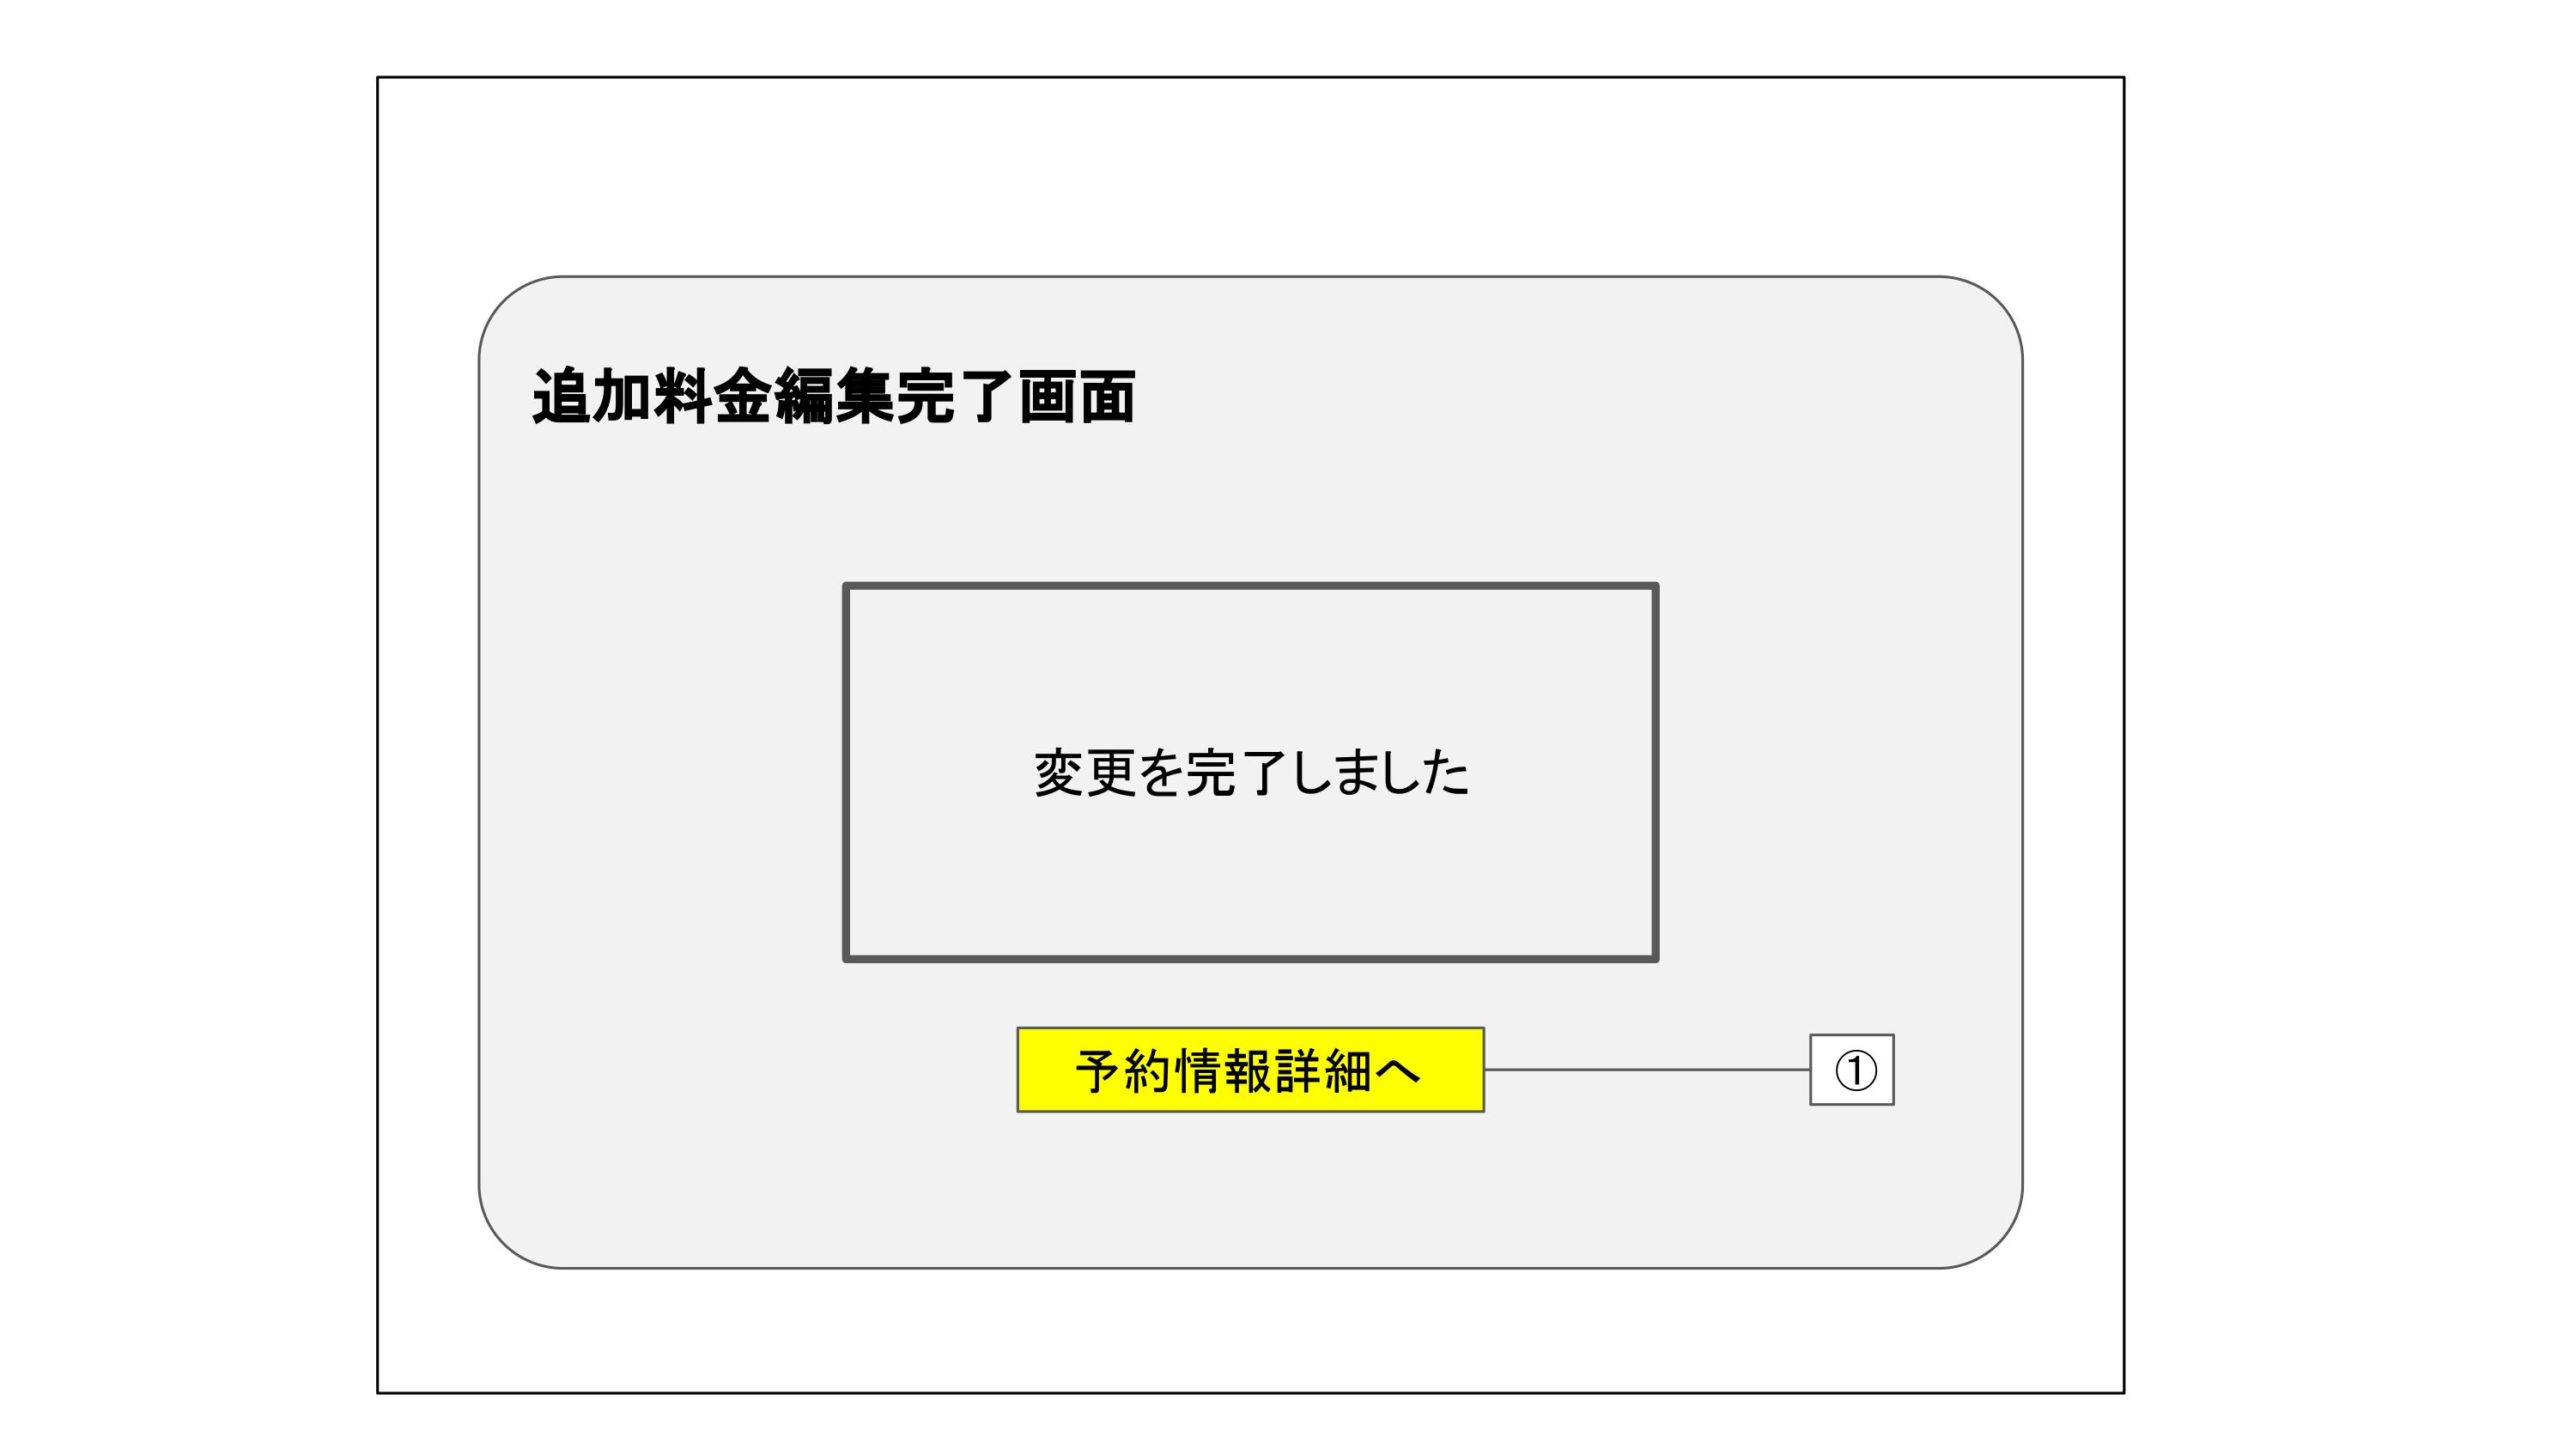
\includegraphics[width=150mm]{UI_front/addfD.jpg}
 \caption{追加料金完了画面}
 \label{fig:frontFc}
\end{figure}

\begin{enumerate}
\renewcommand{\labelenumi}{\textcircled{\scriptsize \theenumi}}
\item 予約情報詳細へ\\ 予約情報詳細へを押すことで,図\ref{fig:frontinf1},図\ref{fig:frontinf2}に示す予約情報詳細画面に遷移する.
\end{enumerate}


\subsubsection{予約検索画面}
 図\ref{fig:frontS}に予約検索画面を示す.

\begin{figure}[H]
 \centering
   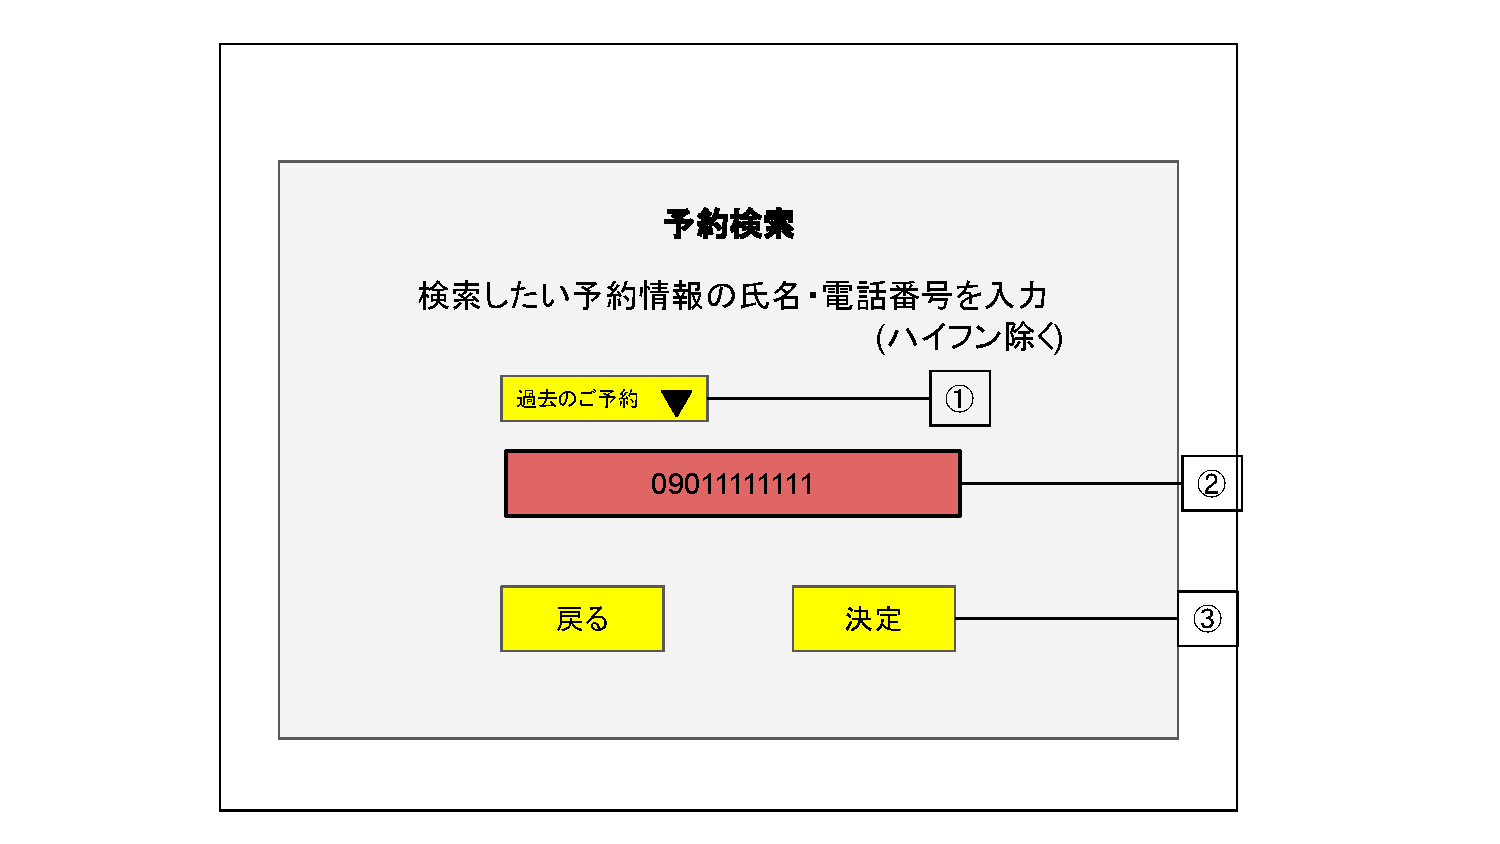
\includegraphics[width=120mm]{UI_front/Reservation-search-screen.pdf}
 \caption{予約検索画面}
 \label{fig:frontS}
\end{figure}

\begin{enumerate}
\renewcommand{\labelenumi}{\textcircled{\scriptsize \theenumi}}
\item 過去のご予約,今後のご予約の選択\\ ドロップダウンリストを押すことで,過去のご予約,今後のご予約を選択する.
\item 氏名/電話番号の入力\\ 赤の欄を押すことで,氏名または電話番号の入力を行う.
\item 決定\\ 決定を押すことで,図\ref{fig:frontSi}に示す予約検索確認画面に遷移する.

\end{enumerate}


\subsubsection{予約検索結果画面}
 図\ref{fig:frontSi}に予約検索結果画面を示す.

\begin{figure}[H]
 \centering
   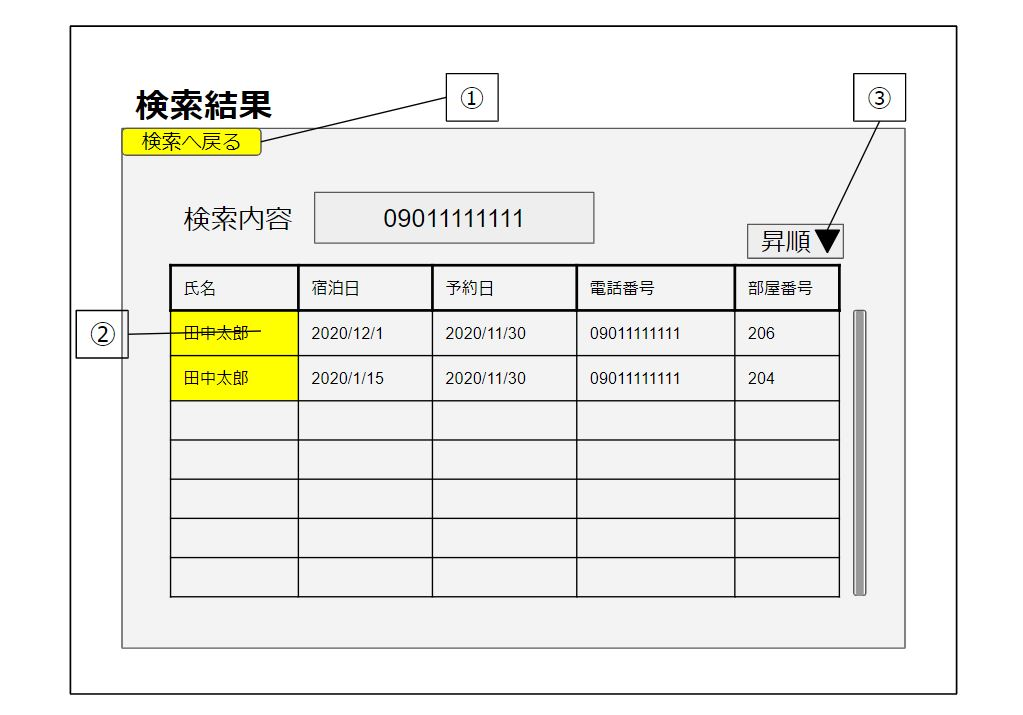
\includegraphics[width=120mm]{UI_front/searchL.jpg}
 \caption{予約検索結果画面}
 \label{fig:frontSi}
\end{figure}

\begin{enumerate}
\renewcommand{\labelenumi}{\textcircled{\scriptsize \theenumi}}
\item 検索へ戻る\\ 検索へ戻るを押すことで,図\ref{fig:frontS}に示す予約検索画面に遷移する.
\item 詳細情報\\ 黄色の氏名を押すことで,図\ref{fig:frontinf1},図\ref{fig:frontinf2}に示す予約情報詳細画面に遷移する.
\item 昇順/降順\\ ドロップダウンリストを押すことで,日付の昇順/降順で並び替える.
\end{enumerate}


\end{document}